\documentclass[egregdoesnotlikesansseriftitles,12pt]{scrartcl}

\usepackage[T1]{fontenc}
\usepackage[utf8]{inputenc}

\usepackage{adjustbox}
\usepackage[affil-it]{authblk}
\usepackage{amssymb}
\usepackage[natbib,authordate,backend=bibtex]{biblatex-chicago}
\usepackage{caption}
\usepackage{color}
\usepackage{enumitem}
\usepackage{flafter}
\usepackage{floatrow}
\usepackage{graphicx}
\usepackage[hidelinks]{hyperref}
\usepackage{multirow}
\usepackage[all]{nowidow}
\usepackage{pdflscape}
\usepackage{setspace}
\usepackage{subcaption}

\newfloatcommand{capbtabbox}{table}[][\FBwidth]

\deffootnote{1.5em}{1em}{\makebox[1.5em][l]{\thefootnotemark}}
   \setlength{\skip\footins}{1.5em}
   \setlength{\footnotesep}{1em}

\captionsetup[subfigure]{labelformat=empty}

\renewcommand\Affilfont{\small}

\renewcommand{\autodot}{}

\urlstyle{same}

\bibliography{references}

\title{Poisoned Babies, Shot Fathers,\\and Ruined Experiments}
\subtitle{Experimental Evidence in Favor of the\\Compositionality Constraint of Actual Causation}

\author[1*]{Alexander Max Bauer}
\author[1]{Stephan Kornmesser}

\affil[1]{ Department of Philosophy, University of Oldenburg}
\affil[*]{ Corresponding Author, E-Mail: \href{mailto:alexander.max.bauer@uni-oldenburg.de}{alexander.max.bauer@uni-oldenburg.de}}

\date{\small \textit{Philosophy of Science} 90 (3), 489--517}

\begin{document}
\maketitle

\begin{abstract}
   \noindent\textbf{Abstract:} Livengood and Sytsma (2020) challenge the Compositionality Constraint of Actual Causation (CCAC), according to which each intermediary of a causal chain is an effect of its predecessor and a cause of its successor link. In several studies, they find support for their hypothesis that the CCAC is not in accordance with ordinary causal attributions of laypeople. We argue that there are three interrelated problems in their studies’ design that we call the Causality-Responsibility Confusion (CRC), the Intermediary-Ontology Confusion (IOC), and the Cause-End Questioning (CEQ). Avoiding the CRC, the IOC, and the CEQ leads to strong empirical support for the CCAC.\\[2ex]
   \textbf{Keywords:} Causation, Compositionality Constraint of Actual Causation, Folk Intuitions, Experimental Philosophy, Vignette Study\\[2ex]
\end{abstract}

\clearpage
\section{Introduction}\label{sec:introduction}
\citet{livengood_actual_2020} (hereafter L\&S 2020) challenge the \textit{Compositionality Constraint of Actual Causation} (CCAC) that is implicitly entailed by many philosophical accounts on actual causation (e.\,g., \cite{reichenbach_direction_1956}; \cite{salmon_causality_1994}; \cite{dowe_causality_1995}, \cite{ehring_causation_1997}; \cite{lewis_causation_1973,lewis_postscripts_1986}; for a brief summary, see L\&S 2020, 43--47). They illustrate the CCAC by a chain of dominos. There are two ways a person could cause the last domino in a chain to fall: First, they could cause it directly by flicking the last domino of the chain. Second, they could cause it indirectly by flicking, for example, the first domino of the chain. It then falls against the second domino, which falls against the third domino and so on, until the last domino of the chain finally falls, too. According to the CCAC, the person causes the last domino to fall in both cases. However, if they do it indirectly, then there must be a number of \textit{intermediaries} -- the falling of one domino against the next one -- such that the person transitively caused the last domino to fall by means of a causal chain.\footnote{Note that the CCAC is (hypothesized to be) a property of causal chains that are to be distinguished from \textit{collider cases} of causation, in which there are two or more direct causes for one and the same effect.} L\&S (2020, 44) formulate the CCAC as follows:

\begin{quote}
   \textsc{CCAC:} If \textit{c} is an actual cause of \textit{e}, then either \textit{c} causes \textit{e} directly or every intermediary \textit{d} by which \textit{c} indirectly causes \textit{e} is itself an actual effect of \textit{c} and an actual cause of \textit{e}.
\end{quote}

\noindent There are two presuppositions to L\&S's (2020) questioning the CCAC. First, they presuppose the \textit{Folk Attribution Desideratum} (FAD) (\cite{livengood_following_2017}), according to which theories of actual causation need to be in accordance with ordinary causal attributions. Hence, the question of whether the CCAC holds becomes a question that can be answered empirically. Second, they presuppose the \textit{Responsibility View} (RV). The RV maintains that the default concept of causation of ordinary causal attributions is a thick concept that also has an evaluative content akin to the concepts \textit{responsibility} and \textit{accountability} (\cite{fischer_causal_2019}; \cite{livengood_following_2017}; \cite{sytsma_two_2012}). This is why ordinary people's judgements of statements like ``$a$ causes $b$'' do not only depend on the question of whether $a$ is a cause of $b$ in a strict sense but also on the question of whether $a$ is responsible for $b$ (\cite{livengood_following_2017}; \cite{knobe_causal_2008}). One could argue against the RV that ordinary people just confuse causation with responsibility and thus give wrong answers.\footnote{The idea that laypeople's views on causation may be influenced by thoughts of responsibility is -- in different forms -- not new; see, e.\,g., \citet{alicke_causation_2011}; \citet{danks_demoralizing_2014}; \citet{samland_how_2016}; \citet{sytsma_causation_2020,sytsma_crossed_2021}.} However, it is not that easy. If one accepts the FAD, one cannot simultaneously state that ordinary people give wrong answers and that the ordinary concept of causation actually does not entail \textit{responsibility}. If data show that ordinary people are significantly more likely to agree to the statement ``$a$ causes $b$'' if $a$ is responsible for $b$, and less likely if $a$ is not responsible for $b$, then the FAD seems to entail the consequence that the concept of causation is a normatively laden concept that contains \textit{responsibility}, and hence that the RV holds.

Presupposing the FAD and the RV, L\&S (2020) challenge the CCAC by surveys based on vignettes in which ``someone or something is responsible for an effect by way of an intermediary that does not share in the responsibility'' (L\&S 2020, 48), such as the following:

\begin{quote}
   \textsc{Poisoned Cup Vignette:} Amy wants to kill her daughter, Jessica, but she doesn't want to go to prison for murder. As such, Amy hatches a plan. She arranges for a baby sitter, Courtney, to take care of Jessica while she is out of town on business. Before leaving, Amy laces one of Jessica's sippy cups with a deadly poison that is very difficult to detect. That evening, Courtney gives Jessica juice in the poisoned sippy cup. Jessica drinks the juice and dies two hours later. (L\&S 2020, 49--51)
\end{quote}

\noindent Presented with the statements

\begin{itemize}
   \item[(1)]\textsc{Amy caused Jessica's death,}
   \item[(2)]\textsc{Courtney caused Jessica's death,}
\end{itemize}

\noindent subjects significantly agree with statement (1) but disagree with statement (2). That is, for causal chains of this kind, subjects tend to accept the if clause of the CCAC because they agree with (1), but they also tend to reject the second conjunct of the or-disjunct of the CCAC because they reject (2). Although the if clause is true, the CCAC seems to be refuted empirically, at least for theories concerned with the \textit{ordinary} concept of causation (L\&S 2020, 64--65). L\&S find support for this finding by nine studies.

In this paper, we will empirically defend the CCAC against L\&S (2020). In Section \ref{sec:theory}, we argue that the refutation of the CCAC presented by L\&S is contestable because of three interrelated problems that we call the \textit{Causality-Responsibility Confusion} (CRC), the \textit{Intermediary-Ontology Confusion} (IOC), and the \textit{Cause-End Questioning} (CEQ). Thereafter, we will show by means of 16 studies that the vignettes of L\&S (2020) lead to results confirming the CCAC if the IOC, the CRC, and the CEQ are avoided.

\section{Three Interrelated Problems of the Supposed Refutation of the Compositionality Constraint of Actual Causation}\label{sec:theory}
In the following, we will introduce three problems that -- to our view -- the design of L\&S (2020) suffers from. According to the CRC (Section \ref{sec:crc}), the design leads subjects to confuse causality with responsibility, which can easily happen in any such study asking for causes in situations that also include instances of responsibility. Ambitions to disentangle causation and responsibility, thus, are of special importance for studies interested in people's evaluations of causation. If we avoid the CRC, we can show that subjects -- contrary to L\&S (2020) -- clearly distinguish between causality and responsibility.

According to the IOC (Section \ref{sec:ioc}), the design of all but one studies of L\&S (2020) uses individuals instead of events as intermediaries of causal chains. We argue that this ontological confusion supports the CRC.

According to the CEQ (Section \ref{sec:ceq}), in each statement that L\&S (2020) ask their subjects to evaluate, the effect of a cause is always the end link of the causal chain presented in the vignette. We argue that the CEQ directly supports the CRC because it triggers responsibility considerations. Further, we argue that the CEQ supports the CRC indirectly because it disguises the IOC, which in turn supports the CRC.

In Section \ref{sec:avoidance}, we provide a brief overview of our studies and explain how we avoid the CRC, the IOC, and the CEQ.

\subsection{The Causality-Responsibility Confusion (CRC)}\label{sec:crc}
The CRC results from the design used by L\&S (2020) that, combined with the IOC (Section \ref{sec:ioc}) and the CEQ (Section \ref{sec:ceq}), leads to a confusion of causation with responsibility or accountability. As \citet{samland_social_2014} already pointed out, in statements of the kind ``$a$ caused $b$'', the verb ``cause'' is ambiguous and might be understood as causation in the narrow sense or as being responsible or accountable, especially in the context of human actions.\footnote{Also consider \citet{schwenkler_cause_nodate} for a series of experiments that avoid using the term ``cause'' in this context. See also \citet{rose_cause_2021}.} The results presented by \citet{samland_social_2014} support their ambiguity hypothesis and hence give rise to the assumption that the statements presented to subjects for evaluation by L\&S (2020) bring about the same ambiguity since all of them are of the form ``$a$ causes $b$''.

However, there are two critical differences to \citet{samland_social_2014}. First, they are only concerned with collider cases of actual causation and not with causal chains as in L\&S (2020). Second, \citet{samland_social_2014} are only concerned with agents causing effects, while L\&S (2020) also present studies with causal chains containing objects or events as causes.

Hence, we will use designs that exclude the ambiguous understanding of ``cause''. However, L\&S could respond to our objection concerning the CRC that we ``might be worried that participants in our study were confusing causation with responsibility. On our view, ordinary people are not confused'' (2020, 52). As causal judgements are sensitive to responsibility considerations, L\&S (2020, 52) conclude that ``the default concept of causation at play in ordinary causal attributions has both descriptive content and normative, evaluative content''. We argue that L\&S confuse the use of the word ``cause'' with the content of the concept \textit{causation}. Of course, we would not argue that ordinary people are confused regarding the use of the word ``cause'' -- they use it as they are used to use it and to use a word in a way that is accepted by the respective linguistic community means to use the word the right way. However, L\&S do not distinguish between the use of the word and the mental representation, i.\,e., the concept of causation. The CCAC is concerned with the concept of causation, and as we will show, ordinary people have a concept of causation which is not ambiguous in the way proposed by L\&S.

\subsection{The Intermediary-Ontology Confusion (IOC)}\label{sec:ioc}
In eight of nine studies of L\&S (2020), the intermediaries of the causal chains are individuals (agents or individual objects) instead of events.\footnote{Only Study 5 of L\&S (2020) presents events instead of individuals as intermediaries.} However, individuals cannot be intermediaries of causal chains. For example, in the Poisoned Cup Vignette, the individual agent Amy is presented as the first link $c$ of the chain, the individual agent Courtney is the intermediary $d$, and the event of Jessica's death is the end link $e$ of the chain. If the agent Courtney were the intermediary, she would have to be the effect of the first link of the chain. Obviously, the agent Courtney is not the effect of the agent Amy, but Courtney's action of giving Jessica juice in a poisoned sippy cup is an effect of Amy's action of poisoning the sippy cup.

Generally speaking: For ontological reasons, individuals (agents or objects) cannot be intermediaries of causal chains. Typically, it is events that are intermediaries of causal chains. Hence, there is an \textit{ontological confusion} concerning the presentation of the intermediaries in all studies but one of L\&S (2020). L\&S could argue that the name ``Courtney'' in statement (2) is only an abbreviation expressing the whole event of giving Jessica juice in a poisoned sippy cup. However, they do not. Instead, they point out that they follow the FAD and that ``one clear finding in recent empirical work on causal attribution is that ordinary people often count agents as causes'' (L\&S 2020, 53). That means that L\&S think they do not need to use events because for ordinary people, individuals can be causes -- even if they are intermediaries of (supposed) causal chains. However, we do not think that ordinary people would accept individuals as intermediary causes of causal chains because individuals cannot be effects of the respective predecessor links of the chains. Otherwise, ordinary people would have to accept statements like ``Amy caused Courtney'' in the case of the Poisoned Cup Vignette or ``The hammer caused the gun powder'' in the case of the Revolver Vignette (see below). It is all the more surprising that L\&S (2020, 44) explicitly introduce the CCAC with respect to events. So why do they choose individuals as intermediaries and, especially, an individual agent as an intermediary in their first and decisive study? An answer to this question might be that they found no differences between individuals and events in being causes in a previous study (see \cite{livengood_following_2017}, 286). However, Livengood, Sytsma, and Rose were concerned with collider cases (in contrast to causal chains) and, hence, the individuals were not \textit{intermediaries} of causal chains (i.e., in the vignettes they were not caused by anything else). Additionally, the phrases denoting the events contained the names of the individuals involved in the event and, thus, emphasize the role of the individual in the respective event.

Contrary to L\&S (2020) we argue that the IOC triggers the Causality-Responsibility Confusion (CRC): Using agents instead of events leads people to understand the verb ``cause'' as \textit{being responsible} for something because only events, not agents, can be causes as intermediaries in causal chains. By contrast, only agents, not events, can be responsible or accountable for something. Hence, the IOC (using agents instead of events as intermediaries) supports the CRC (the confusion of causation with responsibility). For example, with respect to the Poisoned Cup Vignette the IOC supports the subjects' disagreement with the statement that Courtney caused Jessica's death because Courtney is not considered to be responsible for Jessica's death.

If it is true that the CRC is triggered by the IOC, then replacing the agents by events should have an effect on the agreement or disagreement of subjects with the respective statements. However, only in Study 5 L\&S (2020) compare the replacement of agents by events in the statements that are rated by the subjects for the Poisoned Cup Vignette. Here, subjects have to rate their agreement on a 7-point scale with the statements 

\begin{itemize}
   \item[(3)]\textsc{Amy's action of poisoning the sippy cup caused Jessica's death.}
   \item[(4)]\textsc{Courtney's action of giving Jessica juice in the sippy cup caused Jessica's death.}
\end{itemize}

\noindent The disagreement with statement (4) is clearly weaker ($M = 3.36$) than with statement (2) of Study 1 ($M = 2.06$). However, L\&S still conclude that ``[t]he results again suggest that causal attributions of most ordinary people do not satisfy the compositionality constraint'' (2020, 55), because the ratings for the event expressed by (4) is smaller than the scale's neutral value of 4. On the one hand, that is right. On the other hand, it seems obvious that replacing individuals with events as intermediaries in causal chains weakens the refutation of the CCAC. However, stressing the agent Courtney as the actor of the action in statement (4) might trigger the responsibility interpretation of ``cause''. They should have used the statement ``The action of giving Jessica juice in the sippy cup caused Jessica's death''. This statement might achieve an even higher agreement than statement (4), while also avoiding the responsibility interpretation.

We are not the only ones making this point. \citet{samland_how_2016} also remarked that in studies (supposedly) showing that causal judgements are influenced by moral evaluations, the causes are always agents, not events. They assume that ``using the name of an agent as a pointer to an abnormal action possibly creates a context that invites the interpretation of the test question as a request to assess accountability'' (\cite{samland_how_2016}, 171). Their results show a clear difference between statements mentioning and not mentioning individual agents as being involved in the causes expressed by the statements. However, \citet{samland_how_2016} criticize the \textit{Culpable Control Model of Blame} (\cite{alicke_culpable_2000}) and the \textit{Counterfactual Reasoning Account of Causal Selection} (\cite{hitchcock_cause_2009}). They are not concerned with the RV presupposed by L\&S (2020). Further, they are exclusively concerned with collider cases of causation, not with causal chains, and therefore they use different vignettes than L\&S (2020). Hence, we cannot transfer their results to our discussion of the CCAC. Therefore, we will conduct a couple of studies excluding the IOC from the causal chains of the vignettes of L\&S (2020).

However, replacing individuals by events and using events that do not focus on the actor of the respective action of the event is just one piece of the puzzle to resolve the confusions that lead to the refutation of the CCAC. This brings us to the third problem, the CEQ, which -- we think -- simultaneously directly triggers the CRC and supports the IOC.

\subsection{The Cause-End Questioning (CEQ) }\label{sec:ceq}
In all studies of L\&S (2020), subjects are asked to state their agreement with statements of the kind ``$a$ causes $b$'' that work the following way: $b$ is always the end link $e$ of a causal chain presented in the vignettes and $a$ is either the first link $c$ of a causal chain or an intermediary $d$. That is, each statement that is to be rated by subjects of each study of L\&S (2020) expresses a certain cause for the end link $e$ of the causal chain. This is what we call the \textit{Cause-End Questioning} (CEQ). There is no statement in L\&S (2020) expressing that a link $n$ of a causal chain is a cause for the respective next link $n+1$ if the link $n+1$ is not the end of the chain. However, as \citet{bauer_answers_2022} showed for the Revolver Vignette, a more detailed causal chain including more intermediaries leads to a much higher agreement with statements saying that link $n$ is a cause for link $n+1$ (regardless of whether link $n+1$ is the end of the chain or not).

Which effects does the CEQ have? First, in all cases, subjects are asked about their agreement or disagreement only regarding the second conjunct of the or-disjunct of the CCAC (the intermediary $d$ is an actual cause of the end link $e$) but not for the first conjunct (the intermediary $d$ is an effect of the first link $c$). Thus, the CEQ disguises the IOC because it never becomes obvious that the intermediary $d$ cannot be an effect of its predecessor link of the chain if $d$ is an agent. Hence, by disguising the IOC, the CEQ indirectly supports the CRC because the IOC directly supports the CRC (see Section \ref{sec:ioc}). Second, the CEQ directly supports the CRC because each of the end links of the causal chains presented in the vignettes of L\&S (2020) is an undesirable or morally reprehensible event: a poisoned baby, a shot father, or a ruined experiment. Hence, we hypothesize that subjects intuitively look for someone who is responsible for those awful events and, thus, tend to understand the verb ``cause'' as being \textit{responsible}.

Therefore, we think that more detailed chains, in which the intermediaries do not only appear as causes for the end links of the chains but also both as effects of predecessor links and as causes for a further intermediary of the chain, will prevent the problematic effects of the CEQ.

\subsection{How to Exclude the IOC, CRC, and CEQ}\label{sec:avoidance}
In the previous sections, we discussed three problems of L\&S's (2020) refutation of the CCAC that are deeply interrelated: First, the CEQ disguises the IOC and, second, both the IOC and the CEQ support the CRC. In the following, we present our strategy to reevaluate the CCAC that does not fall prey to these problems:

\begin{itemize}
   \item[--]\textsc{Replication:} First, we will replicate L\&S's (2020) initial Studies 1, 8, and 9 on the Poisoned Cup Vignette, the Revolver Vignette, and the GFCI Vignette. In doing so, we will first show that we compare our variations to the same results as obtained by L\&S and, second, that the results of L\&S are not restricted to English and the usage of the English word ``cause'' but are replicable in German with the usage of the respective German word ``verursachen''.
   \item[--]\textsc{IOC Exclusion:} In order to exclude the IOC, we will then use events instead of individuals as intermediaries of causal chains for the Poisoned Cup Vignette, the Revolver Vignette, and the GFCI Vignette. In doing so, we expect to find a higher agreement with the statements referring to events as intermediary causes compared to the statements referring to agents as intermediary causes. However, according to Study 5 of L\&S, we do not expect to find an effect significantly different from the neutral value of 4 by only conducting this modification. Thus, for the Poisoned Cup Vignette we will additionally test the difference between statements mentioning the names of the agents acting in an event and statements not mentioning the names of the agents. In the Revolver Vignette and the GFCI Vignette, there are no agents involved as intermediaries of the causal chains. Hence, we test this variation only for the Poisoned Cup Vignette.
   \item[--]\textsc{CRC Exclusion:} In order to exclude the CRC, we will investigate the ordinary concept of causation without using the word ``cause'' for the Poisoned Cup Vignette, the Revolver Vignette, and the GFCI Vignette. Statements of the kind ``$a$ causes $b$'' tempt to understand ``cause'' as $a$ being responsible or accountable for $b$, especially if $a$ is an agent. Therefore, we will investigate the ordinary concept of causation by, first, replacing the individuals $a$ and $b$ by the statements $\Phi$ and $\Psi$ expressing events and, second, presenting subjects with counterfactual conditionals of the kind ``$\Psi$ would not have happened if $\Phi$ had not happened'', assuming that subjects will agree if the event expressed by $\Phi$ is a cause of the event expressed by $\Psi$.\footnote{A reviewer argued that defenders of the RV would not accept counterfactual conditionals because counterfactual dependence would not be sufficient for actual causation, as they illustrate with the pen case of \citet{knobe_causal_2008}. We agree that the problem depends counterfactually on both actions in the pen case. However, in accordance with \citet{samland_social_2014}, we argue the other way around: Using counterfactual conditionals in the experimental design shows that subject's judgements in \citet{knobe_causal_2008} result from the ambiguous meaning of the verb ``cause'' and, thus, do not reflect their causal representations. Using an experimental design that omits the ambiguous verb and contains counterfactual conditionals instead seems to be more adequate.} However, we are aware of the challenges of \textit{preemption} and \textit{overdetermination} for the counterfactual theory of causation because for cases of preemption and overdetermination, $\Psi$ would also have happened if $\Phi$ had not happened.
   \item[--]\textsc{CEQ Exclusion:} In order to exclude the CEQ, we present statements in which an intermediary $d_{1}$ of a causal chain is an effect of a predecessor link $c$ and, simultaneously, the cause of an effect that is not the end link $e$ of the causal chain but a further intermediary $d_{2}$. We will test this variation for the Poisoned Cup Vignette, the Revolver Vignette, and the GFCI Vignette.
   \item[--]\textsc{Simultaneous IOC, CRC, and CEQ Exclusion}: In a final set of studies, we will exclude the three problems, IOC, CRC, and CEQ, simultaneously for the Poisoned Cup Vignette, the Revolver Vignette, and the GFCI Vignette in order to test whether these variations suppress each other when combined.
\end{itemize}

\section{Design and Procedures}\label{sec:design}
Prior to our main study, we conducted a series of pilot studies with a rather small sample size to test our initial assumptions in the context of one of the vignettes used by L\&S (2020). Details on design, procedure, and results of our pilot studies can be found in Appendix \ref{app:pilot}.

In the main course, we then conducted a total of 16 studies to test the solutions proposed in Section \ref{sec:avoidance}. Here, studies are presented for each vignette separately. For each vignette, we first tried to replicate the original findings from L\&S (2020). Here, the subjects' task was to rate their disagreement or agreement with a number of statements that relate to the vignette's story. This was done on a scale from $1$ (``don't agree at all'') to $7$ (``fully agree'').

Subjects were randomly assigned to one of the 16 studies. Every subject was asked to rate their disagreement or agreement with two, three, or four statements, depending on the respective study. Those statements were all presented on the same screen, together with the vignette's text. Hence, as did L\&S (2020), we presented all statements of a given study to the subjects.

Prior to the vignette and rating task, subjects were greeted with a welcome text (see Appendix \ref{app:main_welcome}). A questionnaire was implemented to appear after the rating task to gain some socio-demographic information.

Furthermore, we asked subjects to answer two to three control questions about the vignette to promote internal validity (see Appendices \ref{app:main_cup_control}, \ref{app:main_revolver_control}, and \ref{app:main_circuit_control}). Only those subjects who answered every question correctly were included in our analysis. Those $1,189$ subjects received a flat fee of $2.10$ euro, which roughly equals an hourly wage of $12.60$ euro. Another $1,370$ subjects were excluded from our analysis after having failed to answer our control questions correctly. As was announced beforehand, they did not receive a compensation.

The studies were programmed in \citet{limesurvey_limesurvey_2021} and conducted online in May 2021. Subjects were recruited by the private market research institute \textit{respondi}, where they have been randomly drawn from a pool of registered subjects from Germany. Hence, the vignettes and statements were presented to them in German.

\section{Results}\label{sec:results}
In the following, we analyze the evaluations made by our subjects.\footnote{Data are available from \url{https://github.com/alephmembeth/causality-compositionality/}.} In Subsection \ref{sec:results_cup}, we first take a look at our studies conducted on the Poisoned Cup Vignette. Thereafter, in Subsection \ref{sec:results_rev}, we investigate the studies on the Revolver Vignette, before turning to the studies regarding the GFCI Vignette in Subsection \ref{sec:results_cir}. Because of space restrictions we mainly focus on the items most interesting for our hypothesis: those containing intermediaries. A more comprehensive list at the end of each subsection, though, contains detailed descriptive information on every item presented to our subjects as well as figures illustrating our results.

\subsection{Poisoned Cup Vignette}\label{sec:results_cup}
First, we present the results of the six different studies conducted on the Poisoned Cup Vignette. Each study introduced the vignette below and asked subjects to rate their agreement with several statements concerning that vignette. 

\begin{quote}
   Gabi wants to kill her daughter, Nele, but she doesn't want to go to prison for murder. As such, Gabi hatches a plan. She arranges for a babysitter, Kathrin, to take care of Nele while she herself is out of town on business. Before leaving, Gabi laces one of Nele's sippy cups with a deadly poison that is very difficult to detect. That evening, Kathrin gives Nele juice in the poisoned sippy cup. Nele drinks the juice and dies two hours later.
\end{quote}

\subsubsection{Replication}\label{sec:results_cup_rep}
The first study's aim was to replicate the findings from L\&S (2020) for the Poisoned Cup Vignette. Figure \ref{fig:cup_rep_bar} shows the mean agreement of our subjects ($N=71$, male: $38$, female: $33$, mean age: $49.169$) with the two statements presented to them:

\begin{itemize}
   \item[(1)]\textsc{Gabi caused Nele's death.}
   \item[(2)]\textsc{Kathrin caused Nele's death.}
\end{itemize}

\noindent As can be seen in Figure \ref{fig:cup_rep_bar} (also see Figures \ref{fig:cup_rep_hist_1} and \ref{fig:cup_rep_hist_2} in Appendix \ref{app:additional_figures} for relative frequencies), the findings from L\&S (2020) were successfully replicated with a German-speaking sample and a German translation of their vignette. Where L\&S (2020, 50) found a mean agreement of $7.00$ with the first statement, we have a mean of $6.859$ ($95\%~CI=[6.679,7.039]$). For the second statement, they found a mean agreement of $2.06$; we have a mean of $2.000$ ($95\%~CI=[1.569,2.431]$). Wilcoxon signed-rank tests further reveal, as was the case in L\&S's study, that the difference to the neutral value of $4$ on the scale from $1$ to $7$ is significant both for the first and the second statement ($p \leq 0.001$).\footnote{Here and in the following, we are not correcting for multiple comparisons.} Following L\&S (2020), this can be seen as an indication of subjects by and large agreeing with the statement that Gabi caused Nele's death, while disagreeing with the statement that Kathrin caused Nele's death. Effect sizes for this are very large in the first ($r=1.166$) and the second ($r=-0.842$) case.\footnote{Effect sizes for Wilcoxon signed-rank tests are calculated by dividing the $z$ value by the square root of $N$. To prevent confusion, we refer to the same ordinary language descriptions as L\&S (2020), following \citet{mcgraw_common_1992}: $|0.0|-|0.2|$ is practically no effect, $|0.2|-|0.4|$ is a small effect, $|0.4|-|0.6|$ is a moderate effect, $|0.6|-|0.8|$ is a large effect, and $\geq |0.8|$ is a very large effect.}

\subsubsection{Exclusion of the Intermediary-Ontology Confusion (IOC) (1)}\label{sec:results_cup_ioc_1}
In order to avoid the IOC, we modified the statements slightly to focus on events instead of agents. This also replicates a modification done by L\&S (2020, 54-55). Subjects ($N=67$, male: $35$, female: $32$, mean age: $48.970$) now had to state their agreement with the statements:

\begin{itemize}
   \item[(1)]\textsc{Gabi's action of poisoning the sippy cup caused Nele's death.}
   \item[(2)]\textsc{Kathrin's action of giving Nele a poisoned sippy cup caused Nele's death.}
\end{itemize}

\noindent As can be seen in Figure \ref{fig:cup_ioc_1_bar} (also see Figures \ref{fig:cup_ioc_1_hist_1} and \ref{fig:cup_ioc_1_hist_2} in Appendix \ref{app:additional_figures} for relative frequencies), the mean agreement with the first sentence remains equally high ($M=6.522$, $95\%~CI=[6.176,6.868]$). The mean agreement with the second statement, though, increases to $3.448$ ($95\%~CI=[2.823,4.072]$). Again, this is very close to the findings from Study 5 of L\&S (2020, 54f.), who report a mean of $6.52$ for the first and of $3.36$ for the second statement. A Wilcoxon signed-rank test indicates that the difference to the neutral value of $4$ remains highly significant for the first statement ($p \leq 0.001$), but no longer for the second one ($p=0.155$). Effect sizes are very large in the first ($r=0.865$) but vanishingly small in the second case ($r=-0.174$). 

In sum, the indication that subjects by and large disagree with the statement that Kathrin caused Nele's death seems to decrease when the singular term referring to Kathrin is replaced by a singular term referring to an event involving Kathrin. However, as we expected in accordance with Study 5 of L\&S (2020), merely excluding the IOC does not lead to an \textit{agreement} with the second statement because of the CRC and the CEQ.

\subsubsection{Exclusion of the Intermediary-Ontology Confusion (IOC) (2)}\label{sec:results_cup_ioc_2}
In a further alteration aiming at avoiding the IOC, we focus on the respective actions without including Gabi's or Kathrin's names into the statements. This time, subjects ($N=81$, male: $34$, female: $55$, mean age: $45.169$) had to state their agreement with the statements:

\begin{itemize}
   \item[(1)]\textsc{The action of poisoning the sippy cup caused Nele's death.}
   \item[(2)]\textsc{The action of giving Nele juice with a poisoned sippy cup caused Nele's death.}
\end{itemize}

\noindent Figure \ref{fig:cup_ioc_2_bar} (also see Figures \ref{fig:cup_ioc_2_hist_1} and \ref{fig:cup_ioc_2_hist_2} in Appendix \ref{app:additional_figures} for relative frequencies) shows that the mean agreement with the second statement further increases ($M=4.640$, $95\%~CI=[4.116,5.164]$). Here, a Wilcoxon signed-rank test shows that the difference to the neutral value of $4$ now becomes significant at the 5\% level for the second statement ($p=0.011$), showing at least a small effect ($r=0.270$). As we hypothesized, replacing a singular term denoting an individual by a singular term referring to an event has a greater influence on the agreement with the second statement if it does not mention an agent.\footnote{A reviewer argued that sentence (2) could be understood as referring to Gabi's instead of Kathrin's action. However, for sentence (2) we used the same verb and the same complements of the verb as in the vignette story. Therefore, we think that there is no reason to assume that subjects confuse Gabi's with Kathrin's action.} We argue that the reason for this is that subjects do not consider the responsibility of the person involved in the event. However, as we expected, we still do not find a clear agreement with the intermediary being a cause of the next link of the causal chain because of the CRC and the CEQ.

\subsubsection{Exclusion of the Causality-Responsibility Confusion (CRC)}\label{sec:results_cup_crc}
In order to outwit the CRC, we rephrased the statements as counterfactual conditionals avoiding the term ``cause''. Here, subjects ($N=86$, male: $40$, female: $46$, mean age: $43.256$) had to state their agreement with the sentences:

\begin{itemize}
   \item[(1)]\textsc{Nele would not have died that evening if Gabi had not poisoned her sippy cup.}
   \item[(2)]\textsc{Nele would not have died that evening if Kathrin had not given her juice in a poisoned sippy cup.}
\end{itemize}

\noindent Figure \ref{fig:cup_crc_bar} (also see Figures \ref{fig:cup_crc_hist_1} and \ref{fig:cup_crc_hist_2} in Appendix \ref{app:additional_figures} for relative frequencies) shows that the mean agreement with the second statement clearly increases further ($M=5.953$, $95\%~CI=[5.548,6.359]$). A Wilcoxon signed-rank test reveals that now the difference to the neutral value of $4$ is highly significant for this statement ($p \leq 0.001$), showing a large effect ($r=0.724$). We take this to be strong evidence in favor of our hypothesis that excluding the CRC by avoiding the use of the ambiguous word ``cause'' supports the CCAC. Presenting statements with counterfactual conditionals enables an investigation of the ordinary \textit{concept} of causation and prevents producing misleading evidence concerning the ordinary uses of the ambiguous \textit{word} ``cause''.

\subsubsection{Exclusion of the Cause-End Questioning (CEQ)}\label{sec:results_cup_ceq}
In order to avoid the CEQ, we introduced the further intermediary of Nele's action of ingesting poison to the causal chain. Hence, we presented the following three statements to subjects ($N=61$, male: $27$, female: $34$, mean age: $48.295$):

\begin{itemize}
   \item[(1)]\textsc{Gabi's action of poisoning Nele's sippy cup caused Kathrin to give Nele juice in a poisoned sippy cup.}
   \item[(2)]\textsc{Kathrin's action of giving Nele juice in a poisoned sippy cup caused Nele to ingest poison.}
   \item[(3)]\textsc{Nele's action of ingesting poison caused her death.}
\end{itemize}

\noindent The mean agreement with every statement is higher than the neutral value of 4, as can be seen in Figure \ref{fig:cup_ceq_bar} (also see Figures \ref{fig:cup_ceq_hist_1}, \ref{fig:cup_ceq_hist_2}, and \ref{fig:cup_ceq_hist_3} in Appendix \ref{app:additional_figures} for relative frequencies). Again, we are mainly interested in the second statement because we introduced a further intermediary of which Kathin's action of giving Nele juice in a poisoned sippy cup is the cause. For the second statement, the mean agreement is at $5.115$ ($95\%~CI=[4.501,5.728]$). A Wilcoxon signed-rank test shows that the difference to the neutral value of $4$ is highly significant for this statement ($p \leq 0.001$), with a moderate effect ($r=0.437$). We expected that changing the effect of Kathrin's action to a less undesirable event would reduce the support of the CEQ to the CRC and, thus, would lead to a higher agreement. We found that even if the effect is only slightly less undesirable -- causing someone to ingest poison might be only slightly better than causing someone to die -- there is a highly significant agreement with the second statement as opposed to the agreement with the second statement of the replication. Thus, excluding the CEQ shows a clear effect supporting the CCAC contrary to L\&S (2020).

\subsubsection{Simultaneous IOC, CRC, and CEQ Exclusion}\label{sec:results_cup_com}
Lastly, a set of subjects ($N=59$, male: $30$, female: $29$, mean age: $45.610$) was presented with sentences that combined the previous approaches. They had to state their agreement with the sentences:

\begin{itemize}
   \item[(1)]\textsc{Kathrin would not have given Nele juice in a poisoned sippy cup if Gabi had not poisoned Nele's sippy cup.}
   \item[(2)]\textsc{Nele would not have ingested poison if Kathrin had not given her juice in a poisoned sippy cup.}
   \item[(3)]\textsc{Nele would not have died that evening if she had not ingested the poison.}
\end{itemize}

\noindent The mean agreement with every statement is higher than the neutral value of 4, as can be seen in Figure \ref{fig:cup_com_bar} (also see Figures \ref{fig:cup_com_hist_1}, \ref{fig:cup_com_hist_2}, and \ref{fig:cup_com_hist_3} in Appendix \ref{app:additional_figures} for relative frequencies). The second statement is evaluated at $6.169$ ($95\%~CI=[5.695,6.644]$). A Wilcoxon signed-rank test shows that the difference to the neutral value of $4$ is highly significant for the second case ($p \leq 0.001$), exhibiting a large effect ($r=0.757$). Again, the agreement with the second statement with Kathrin's action being the cause of the next link of the chain is of special interest to us. It has the highest agreement of all statements with Kathrin's action being a cause. Clearly, the modifications IOC Exclusion, CRC Exclusion, and CEQ Exclusion do not suppress and might even support one another.

\subsubsection{Summary}\label{sec:results_cup_sum}
Figure \ref{fig:cup} shows the means of our subjects' agreements to the respective statements for the Replication (Figure \ref{fig:cup_rep_bar}), the first (Figure \ref{fig:cup_ioc_1_bar}) and second (Figure \ref{fig:cup_ioc_2_bar}) IOC Exclusion, the CRC Exclusion (Figure \ref{fig:cup_crc_bar}), the CEQ Exclusion (Figure \ref{fig:cup_ceq_bar}), as well as the Simultaneous IOC, CRC, and CEQ Exclusion (Figure \ref{fig:cup_com_bar}). Additionally, Table \ref{tab:cup_statements} summarizes the statements presented in our studies on the Poisoned Cup Vignette. Beyond the modifications IOC Exclusion (1) and (2), we can see a highly significant agreement with the second statement of each study, considering the intermediary to be a cause in the causal chain contrary to L\&S (2020). Further, the two-sample Wilcoxon rank-sum tests comparing the statements of our modifications to those of our replication (right column) show that the second statement of each modification is evaluated significantly different compared to our replication in each and every subsequent study. We take our results to be strong evidence in favor of the CCAC -- contrary to the original findings of L\&S (2020). The design of L\&S (2020), we suppose, leads subjects to understand the word ``cause'' as ``being responsible for'' and, hence, not to agree with statements expressing that agents who do not share in the responsibility are causes. However, excluding the CRC by avoiding the ambiguous word ``cause'' as well as the IOC and the CEQ both supporting the CRC leads for the same vignette as used by L\&S to strong evidence in favor of the CCAC.

\begin{landscape}
\begin{figure}[h!]
   \begin{subfigure}[t]{0.28\textwidth}
      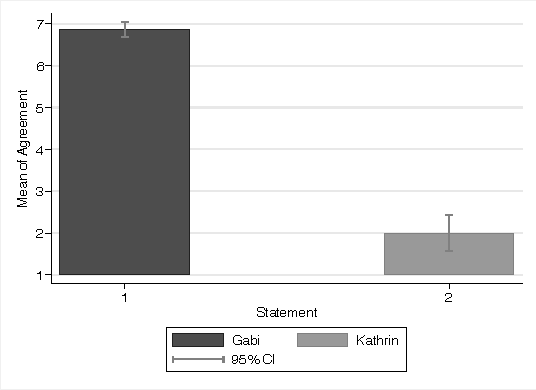
\includegraphics[scale=0.7]{figures/cup_rep_bar.pdf}
      \caption{\textsf{\scriptsize(a) Replication}}
      \label{fig:cup_rep_bar}
   \end{subfigure}
   \begin{subfigure}[t]{0.28\textwidth}
      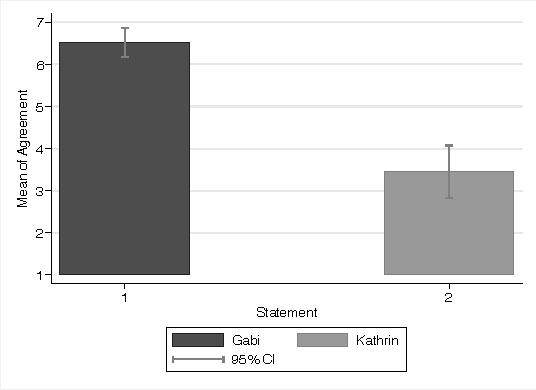
\includegraphics[scale=0.7]{figures/cup_ioc_1_bar.pdf}
      \caption{\textsf{\scriptsize(b) IOC Exclusion (1)}}
      \label{fig:cup_ioc_1_bar}
   \end{subfigure}
   \begin{subfigure}[t]{0.28\textwidth}
      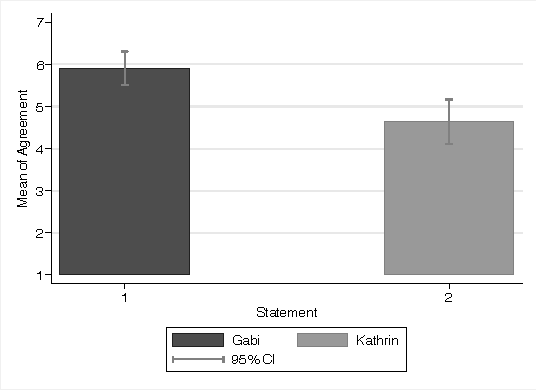
\includegraphics[scale=0.7]{figures/cup_ioc_2_bar.pdf}
      \caption{\textsf{\scriptsize(c) IOC Exclusion (2)}}
      \label{fig:cup_ioc_2_bar}
   \end{subfigure}
   \begin{subfigure}[t]{0.28\textwidth}
      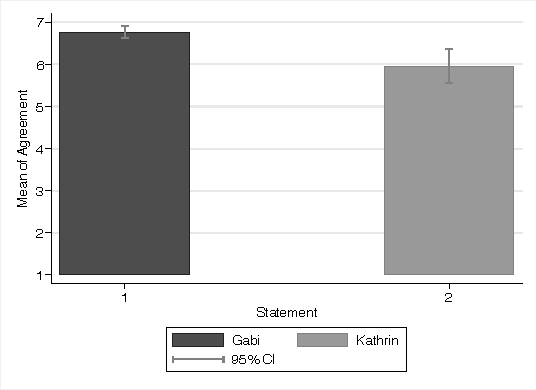
\includegraphics[scale=0.7]{figures/cup_crc_bar.pdf}
      \caption{\textsf{\scriptsize(d) CRC Exclusion}}
      \label{fig:cup_crc_bar}
   \end{subfigure}
   \begin{subfigure}[t]{0.28\textwidth}
      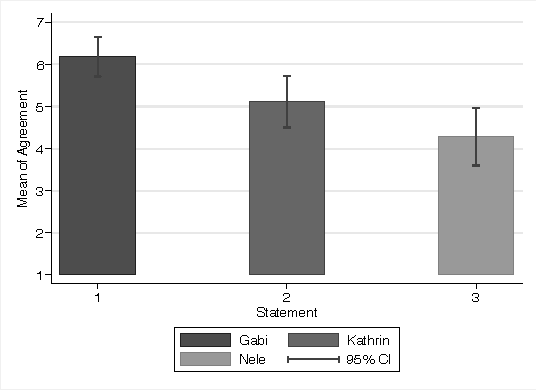
\includegraphics[scale=0.7]{figures/cup_ceq_bar.pdf}
      \caption{\textsf{\scriptsize(e) CEQ Exclusion}}
      \label{fig:cup_ceq_bar}
   \end{subfigure}
   \begin{subfigure}[t]{0.28\textwidth}
      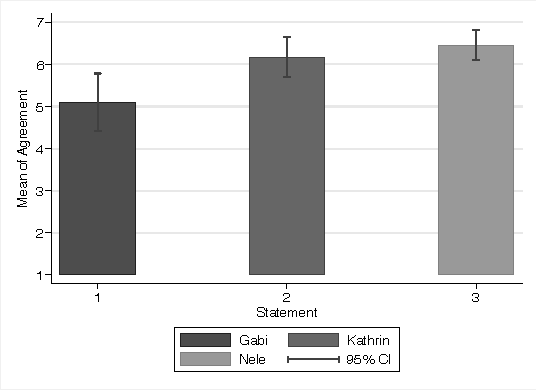
\includegraphics[scale=0.7]{figures/cup_com_bar.pdf}
      \caption{\textsf{\scriptsize(f) Simultaneous IOC, CRC, and CEQ Exclusion}}
      \label{fig:cup_com_bar}
   \end{subfigure}
   \caption{Means of agreements for the Replication (\ref{fig:cup_rep_bar}), the first (\ref{fig:cup_ioc_1_bar}) and second (\ref{fig:cup_ioc_2_bar}) IOC Exclusion, the CRC Exclusion (\ref{fig:cup_crc_bar}), the CEQ Exclusion (\ref{fig:cup_ceq_bar}), as well as the Simultaneous IOC, CRC, and CEQ Exclusion (\ref{fig:cup_com_bar}) with the Poisoned Cup Vignette}\label{fig:cup}
\end{figure}
\end{landscape}

\begin{landscape}
\begin{table}[]
\resizebox{\linewidth}{!}{%
\begin{tabular}{lrlcccccccccc}
   \hline
                                  &                     &                                                                                                                                                                         &                         &           &                   &   & \multicolumn{3}{c}{Versus Neutral Value}       &   & \multicolumn{2}{c}{Versus Replication}   \\\cline{8-10}\cline{12-13}
   Study                          &                     & Statement                                                                                                                                                               & $N$                     & $M$       & $95\%~CI$         &   & $z$        & $p$                  & $r$        &   & $z$        & $p$                         \\
   \hline\hline
   \multirow{2}{*}{Replication}   & \footnotesize (1)   & \footnotesize ``Gabi caused Nele's death.''                                                                                                                             & \multirow{2}{*}{$71$}   & $6.859$   & $[6.679,7.039]$   &   & $ 8.242$   & $\leq 0.001^{***}$   & $ 1.166$   &   & $-$        & $-$                         \\
                                  & \footnotesize (2)   & \footnotesize ``Kathrin caused Nele's death.''                                                                                                                          &                         & $2.000$   & $[1.569,2.431]$   &   & $-5.952$   & $\leq 0.001^{***}$   & $-0.842$   &   & $-$        & $-$                         \\
   \hline
   \multirow{2}{*}{IOC (1)}       & \footnotesize (1)   & \footnotesize\begin{tabular}[c]{@{}l@{}}``Gabis's action of poisoning the\\ sippy cup caused Nele's death.''\end{tabular}                                               & \multirow{2}{*}{$67$}   & $6.522$   & $[6.176,6.868]$   &   & $ 7.076$   & $\leq 0.001^{***}$   & $ 0.865$   &   & $ 1.918$   & $0.055$                     \\
                                  & \footnotesize (2)   & \footnotesize\begin{tabular}[c]{@{}l@{}}``Kathrin's action of giving Nele a\\ poisoned sippy cup caused Nele's death.''\end{tabular}                                    &                         & $3.447$   & $[2.823,4.072]$   &   & $-1.424$   & $0.155$              & $-0.174$   &   & $-3.587$   & $\leq 0.001^{***}$          \\
   \hline
   \multirow{2}{*}{IOC (2)}       & \footnotesize (1)   & \footnotesize\begin{tabular}[c]{@{}l@{}}``The action of poisoning the sippy cup\\ caused Nele's death.''\end{tabular}                                                   & \multirow{2}{*}{$89$}   & $5.910$   & $[5.514,6.306]$   &   & $ 6.648$   & $\leq 0.001^{***}$   & $ 0.705$   &   & $ 4.333$   & $\leq 0.001^{***}$          \\
                                  & \footnotesize (2)   & \footnotesize\begin{tabular}[c]{@{}l@{}}``The action of giving Nele juice with a\\ poisoned sippy cup caused Nele's death.''\end{tabular}                               &                         & $4.640$   & $[4.116,5.164]$   &   & $ 2.551$   & $0.011$              & $ 0.270$   &   & $-6.441$   & $\leq 0.001^{***}$          \\
   \hline
   \multirow{2}{*}{CRC}           & \footnotesize (1)   & \footnotesize\begin{tabular}[c]{@{}l@{}}``Nele would not have died that evening if\\ Gabi had not poisoned her sippy cup.''\end{tabular}                                & \multirow{2}{*}{$86$}   & $6.767$   & $[6.618,6.917]$   &   & $ 8.783$   & $\leq 0.001^{***}$   & $ 0.947$   &   & $ 1.812$   & $0.070$                     \\
                                  & \footnotesize (2)   & \footnotesize\begin{tabular}[c]{@{}l@{}}``Nele would not have died that evening if\\ Kathrin had not given her juice in a poisoned sippy cup.''\end{tabular}            &                         & $5.953$   & $[5.548,6.359]$   &   & $ 6.716$   & $\leq 0.001^{***}$   & $ 0.724$   &   & $-8.927$   & $\leq 0.001^{***}$          \\
   \hline
   \multirow{3}{*}{CEQ}           & \footnotesize (1)   & \footnotesize\begin{tabular}[c]{@{}l@{}}``Gabi's action of poisoning Nele's sippy cup\\ caused Kathrin to give Nele juice in a poisoned sippy cup.''\end{tabular}       & \multirow{3}{*}{$61$}   & $6.180$   & $[5.714,6.649]$   &   & $ 6.145$   & $\leq 0.001^{***}$   & $ 0.787$   &   & $ 2.812$   & $0.005^{**}$                \\
                                  & \footnotesize (2)   & \footnotesize\begin{tabular}[c]{@{}l@{}}``Kathrin's action of giving Nele juice in a\\ poisoned sippy cup caused Nele to ingest poison.''\end{tabular}                  &                         & $5.115$   & $[4.501,5.728]$   &   & $ 3.413$   & $\leq 0.001^{***}$   & $ 0.437$   &   & $-6.678$   & $\leq 0.001^{***}$          \\
                                  & \footnotesize (3)   & \footnotesize ``Nele's action of ingesting poison caused her death.''                                                                                                   &                         & $4.279$   & $[3.599,4.958]$   &   & $ 0.596$   & $0.551$              & $ 0.076$   &   & $-$        & $-$                         \\
   \hline
   \multirow{3}{*}{Combination}   & \footnotesize (1)   & \footnotesize\begin{tabular}[c]{@{}l@{}}``Kathrin would not have given Nele juice in a poisoned sippy cup if\\ Gabi had not poisoned Nele's sippy cup.''\end{tabular}   & \multirow{3}{*}{$59$}   & $5.102$   & $[4.421,5.782]$   &   & $ 2.969$   & $0.003^{**}$         & $ 0.387$   &   & $ 5.008$   & $\leq 0.001^{***}$          \\
                                  & \footnotesize (2)   & \footnotesize\begin{tabular}[c]{@{}l@{}}``Nele would not have ingested poison if\\ Kathrin had not given her juice in a poisoned sippy cup.''\end{tabular}              &                         & $6.169$   & $[5.695,6.644]$   &   & $ 5.814$   & $\leq 0.001^{***}$   & $ 0.757$   &   & $-8.237$   & $\leq 0.001^{***}$          \\
                                  & \footnotesize (3)   & \footnotesize\begin{tabular}[c]{@{}l@{}}``Nele would not have died that evening if\\ she had not ingested the poison.''\end{tabular}                                    &                         & $6.458$   & $[6.101,6.814]$   &   & $ 6.609$   & $\leq 0.001^{***}$   & $ 0.860$   &   & $-$        & $-$                         \\
   \hline\\[-1.5ex]
   \multicolumn{13}{p{26cm}}{\footnotesize\textit{$N$ gives the number of participants for each study. Thereafter, the mean agreement ($M$) and 95\% Confidence Intervals ($95\%~CI$) are given for every statement. Furthermore, the results of Wilcoxon signed-rank tests comparing the agreement with each statement with the neutral value of $4$ are reported, followed by the Effect Size ($r$), calculated by dividing the $z$ value by the square root of $N$. Additionally, two-sample Wilcoxon rank-sum tests are reported comparing the statements from subsequent studies to those from our replication. Asterisks denote significance levels: $^{*}p\le0.05$, $^{**}p\le0.01$, $^{***}p\le0.001$.}}
   \caption{Summary of Statements for the Poisoned Cup Vignette}\label{tab:cup_statements}
\end{tabular}}
\end{table}
\end{landscape}

\subsection{Revolver Vignette}\label{sec:results_rev}
Next, we take a look at another five studies that were conducted with the following Revolver Vignette: 

\begin{quote}
   Leeve has decided to kill his father, Uwe. He aims his loaded revolver at Uwe and pulls the trigger, releasing the hammer. The hammer strikes the cartridge, igniting the gun powder. The gun powder explodes, driving the bullet from the gun. The bullet hits Uwe in the head. He dies instantly.
\end{quote}

\subsubsection{Replication}\label{sec:results_rev_rep}
The first study aimed at replicating the findings from L\&S (2020) for the Revolver Vignette. Here, subjects ($N=63$, male: $26$, female: $37$, mean age: $40.095$) had to state their agreement with the statements:

\begin{itemize}
   \item[(1)]\textsc{Leeve caused Uwe's death.}
   \item[(2)]\textsc{The hammer caused Uwe's death.}
   \item[(3)]\textsc{The gun powder caused Uwe's death.}
   \item[(4)]\textsc{The bullet caused Uwe's death.}
\end{itemize}

\noindent The mean agreement with the first statement from L\&S (2020, 60) is $6.705$; our mean is at at $6.603$ ($95\%~CI=[6.285,6.922]$), as can be seen in Figure \ref{fig:rev_rep_bar} (also see Figures \ref{fig:rev_rep_hist_1}, \ref{fig:rev_rep_hist_2}, \ref{fig:rev_rep_hist_3}, and \ref{fig:rev_rep_hist_4} in Appendix \ref{app:additional_figures} for relative frequencies). Statement (2) has a mean of $2.490$ in the original; our mean is at $3.000$. The third statement's original mean is $2.275$; we find a mean of $2.984$. Lastly, L\&S (2020) found a mean of $4.373$ for the fourth statement; we have a mean of $5.048$.\footnote{L\&S (2020, 60) only report the mean for the first statement. We are thankful to them for sharing their data with us so that we can report the original means for all four statements.} Wilcoxon signed-rank tests show that the first three statements from L\&S (2020) are significantly different from the neutral value of four.\footnote{Statement 1: $z=6.464$, $p \leq 0.001$; Statement 2: $z=-4.068$, $p \leq 0.001$; Statement 3: $z=-4.732$, $p \leq 0.001$; Statement 4: $z= 0.847$, $p=0.397$.} The same holds true for our first ($z=7.108$, $p \leq 0.001$), second ($z=-3.288$, $p \leq 0.001$), and third statement ($z=-3.391$, $p \leq 0.001$). Only the last statement is evaluated different from the original study; here we find a significant deviation from the neutral value of 4 at the 1\% level ($z=2.826$, $p=0.005$) where L\&S find none. Overall, this suggests that subjects by and large agree with the statement that Leeve (or Trent in the original vignette) caused the death of Uwe (or Brad in the original vignette). At the same time they disagree with the statements that the hammer or the gunpowder caused Uwe's (or Brad's) death. Despite the slightly different means we can consider this as a successful replication of the original study. In the following, we will focus on the statements (2) and (3) mentioning intermediaries that, contrary to the CCAC, are not rated to be causes in L\&S (2020) and in our replication.

\subsubsection{Exclusion of the Intermediary-Ontology Confusion (IOC)}\label{sec:results_rev_ioc}
The second study rephrased the statements to avoid the IOC. Subjects had to evaluate the statements:

\begin{itemize}
   \item[(1)]\textsc{Leeve's action of shooting at Uwe caused Uwe's death.}
   \item[(2)]\textsc{The release of the hammer caused Uwe's death.}
   \item[(3)]\textsc{The explosion of the gun powder caused Uwe's death.}
   \item[(4)]\textsc{The bullet hitting Uwe caused Uwe's death.}
\end{itemize}

\noindent The responses to statements (2) and (3) are of special interest to us because subjects tended to disagree with them originally. As can be seen in Figure \ref{fig:rev_ioc_bar} (also see Figures \ref{fig:rev_ioc_hist_1}, \ref{fig:rev_ioc_hist_2}, \ref{fig:rev_ioc_hist_3}, and \ref{fig:rev_ioc_hist_4} in Appendix \ref{app:additional_figures} for relative frequencies), subjects ($N=54$, male: $26$, diverse: $1$, female: $27$, mean age: $41.704$) state a mean agreement of $3.667$ ($95\%~CI=[2.988,4.346]$) to the second and of $3.593$ ($95\%~CI=[2.917,4.269]$) to the third statement. Wilcoxon signed-rank tests show that, in contrast to the replication above, the mean agreement with the second ($p=0.357$) and third ($p=0.219$) statements are no longer evaluated significantly different from 4. Here, effect sizes are vanishingly small, though ($r=-0.125$, $r=-0.167$). It seems we can no longer infer that subjects would disagree with the statements that the release of the hammer or the explosion of the gunpowder caused Uwe's death. That is, as expected we see the same effect of the IOC Exclusion for those statements subjects tended to disagree with in the replication as in the Poisoned Cup Vignette: Excluding the IOC leads subjects not to disagree with statements they tended to disagree with when the IOC was not excluded.

\subsubsection{Exclusion of the Causality-Responsibility Confusion (CRC)}\label{sec:results_rev_crc}
In a third study, subjects ($N=50$, male: $18$, female: $32$, mean age: $42.980$) were presented with counterfactual conditionals that omitted the word ``cause'' to avoid the CRC. We asked them to rate the statements:

\begin{itemize}
   \item[(1)]\textsc{Uwe would not have died if Leeve had not shot at him.}
   \item[(2)]\textsc{Uwe would not have died if the hammer had not been released.}
   \item[(3)]\textsc{Uwe would not have died if the gun powder had not exploded.}
   \item[(4)]\textsc{Uwe would not have died if the bullet had not hit Uwe.}
\end{itemize}

\noindent As can be seen in Figure \ref{fig:rev_crc_bar} (also see Figures \ref{fig:rev_crc_hist_1}, \ref{fig:rev_crc_hist_2}, \ref{fig:rev_crc_hist_3}, and \ref{fig:rev_crc_hist_4} in Appendix \ref{app:additional_figures} for relative frequencies), mean agreements with statements (2) and (3) are now distinctly higher than the neutral value of $4$. For the second statement, it is at $6.12$ ($95\%~CI=[5.582,6.658]$), for the third at $5.720$ ($95\%~CI=[5.110,6.330]$). Wilcoxon signed-rank tests show that the mean agreement with statements (2) and (3) is indeed significantly different from the neutral value ($p \leq 0.001$). Effect sizes are large for both statements ($r=0.755$, $r=0.631$). By excluding the CRC, we found subjects to strongly agree that both the release of the hammer and the explosion of the gun powder are causes in the causal chain. As in the Poisoned Cup Vignette, we take this to be strong evidence in favor of our hypothesis that excluding the CRC by avoiding the use of the ambiguous word ``cause'' supports the CCAC. Presenting statements with counterfactual conditionals enables an investigation of the ordinary \textit{concept} of causation and prevents producing misleading evidence concerning the ordinary uses of the ambiguous \textit{word} ``causation''.

\subsubsection{Exclusion of the Cause-End Questioning (CEQ)}\label{sec:results_rev_ceq}
Next, we constructed a causal chain for the Revolver Vignette to avoid the CEQ. Here, subjects were shown the statements:

\begin{itemize}
   \item[(1)]\textsc{Leeve's action of shooting at Uwe caused the release of the hammer.}
   \item[(2)]\textsc{The release of the hammer caused the explosion of the gun powder.}
   \item[(3)]\textsc{The explosion of the gun powder caused the bullet to hit Uwe.}
   \item[(4)]\textsc{The bullet hitting Uwe caused Uwe's death.}
\end{itemize}

\noindent Subjects' ($N=53$, male: $23$, female: $30$, mean age: $40.774$) mean agreements with statements (2) and (3) were again above 4, as can be seen in Figure \ref{fig:rev_ceq_bar} (also see Figures \ref{fig:rev_ceq_hist_1}, \ref{fig:rev_ceq_hist_2}, \ref{fig:rev_ceq_hist_3}, and \ref{fig:rev_ceq_hist_4} in Appendix \ref{app:additional_figures} for relative frequencies). The mean agreement with the second statement was at $5.830$ ($95\%~CI=[5.272,6.389]$), with the third at $5.057$ ($95\%~CI=[4.396,5.717]$). Wilcoxon signed-rank tests show that the mean agreement is significantly different from the neutral value ($p \leq 0.001$, $p=0.003$). Here, effect sizes are large in the second ($r=0.675$) and moderate in the third ($r=0.404$) case. Compared to the disagreements with the statements (2) and (3) of the replication, subjects now tend to agree that the release of the hammer and the explosion of the gun powder are causes in a causal chain. Thus, excluding the CEQ shows a clear effect in support of the CCAC.

\subsubsection{Simultaneous IOC, CRC, and CEQ Exclusion}\label{sec:results_rev_com}
Lastly, we presented a combination of the previous approaches. Here, subjects were given the statements:

\begin{itemize}
   \item[(1)]\textsc{The hammer would not have released if Leeve had not shot at Uwe.}
   \item[(2)]\textsc{The gun powder would not have exploded if the hammer had not released.}
   \item[(3)]\textsc{The bullet would not have hit Uwe if the gun powder had not exploded.}
   \item[(4)]\textsc{Uwe would not have died if the bullet had not hit Uwe.}
\end{itemize}

\noindent Once more, the mean agreements of our subjects ($N=50$, male: $30$, diverse: $1$, female: $18$, mean age: $44.740$) with the statements (2) and (3) were above $4$, even above $6$, as depicted in Figure \ref{fig:rev_com_bar} (also see Figures \ref{fig:rev_com_hist_1}, \ref{fig:rev_com_hist_2}, \ref{fig:rev_com_hist_3}, and \ref{fig:rev_com_hist_4} in Appendix \ref{app:additional_figures} for relative frequencies). Specifically, the mean agreement with the second statement is at $6.520$ ($95\%~CI=[6.194,6.846]$) and with the third at $6.12$ ($95\%~CI=[5.680,6.560]$). Wilcoxon signed-rank tests show that here, too, the mean agreement is significantly different from the neutral value ($p \leq 0.001$). Effect sizes are very large for the second ($r=0.856$) and large for the third case ($r=0.786$). Thus, we find the highest agreements for the release of the hammer and the explosion of the gun powder being causes in the causal chain. Obviously, the IOC Exclusion, CRC Exclusion, and CEQ Exclusion do not suppress and might even support each other.

\subsubsection{Summary}\label{sec:results_rev_sum}
Figure \ref{fig:rev} shows the means of our subjects' agreements to the respective statements for the Replication (Figure \ref{fig:rev_rep_bar}), the IOC Exclusion (Figure \ref{fig:rev_ioc_bar}), the CRC Exclusion (Figure \ref{fig:rev_crc_bar}), the CEQ Exclusion (Figure \ref{fig:rev_ceq_bar}), as well as the Simultaneous IOC, CRC, and CEQ Exclusion (Figure \ref{fig:rev_com_bar}). Additionally, Table \ref{tab:rev_statements} summarizes the statements presented in our studies on the Revolver Vignette. Beyond the IOC Exclusion, we can see significant or highly significant agreements with the statements (2) and (3) in each study with effect sizes being large or very large in all cases except one with a moderate effect size. Further, the two-sample Wilcoxon rank-sum tests comparing the statements of our modifications to those of our replication (right column) show that the statements (2) and (3) of each modification beyond the IOC Exclusion are evaluated significantly different compared to our replication in each and every subsequent study. Hence, we take our results to be strong evidence in favor of the CCAC. 

\begin{landscape}
\begin{figure}[h!]
   \begin{subfigure}[t]{0.28\textwidth}
      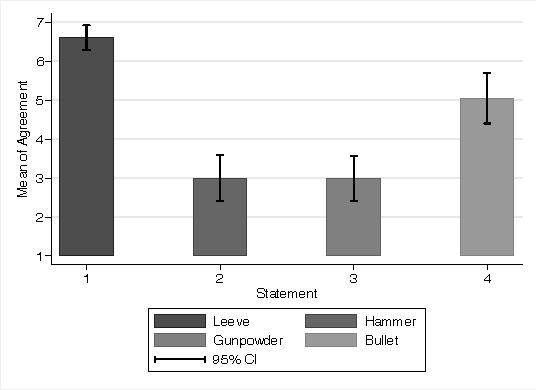
\includegraphics[scale=0.7]{figures/rev_rep_bar.pdf}
      \caption{\textsf{\scriptsize(a) Replication}}
      \label{fig:rev_rep_bar}
   \end{subfigure}
   \begin{subfigure}[t]{0.28\textwidth}
      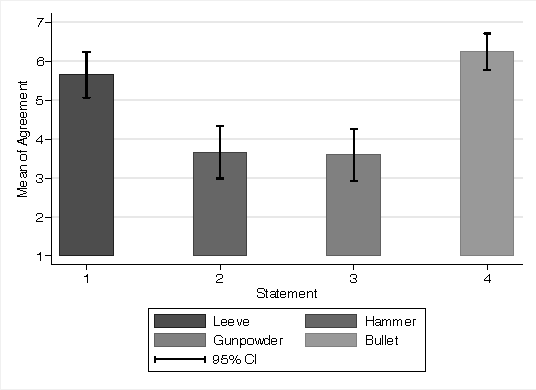
\includegraphics[scale=0.7]{figures/rev_ioc_bar.pdf}
      \caption{\textsf{\scriptsize(b) IOC Exclusion}}
      \label{fig:rev_ioc_bar}
   \end{subfigure}
   \begin{subfigure}[t]{0.28\textwidth}
      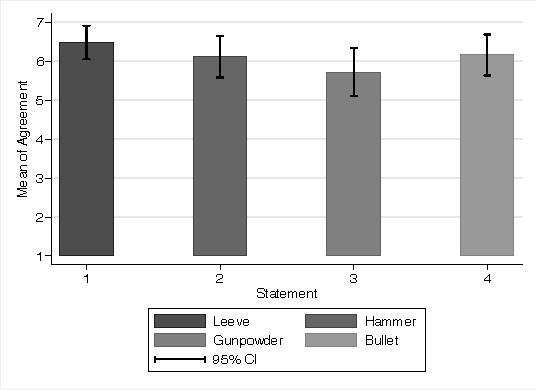
\includegraphics[scale=0.7]{figures/rev_crc_bar.pdf}
      \caption{\textsf{\scriptsize(c) CRC Exclusion}}
      \label{fig:rev_crc_bar}
   \end{subfigure}
   \begin{subfigure}[t]{0.28\textwidth}
      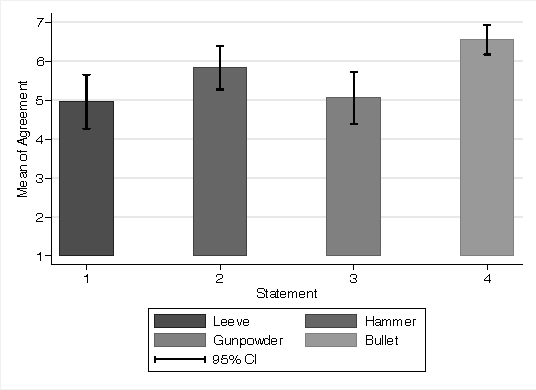
\includegraphics[scale=0.7]{figures/rev_ceq_bar.pdf}
      \caption{\textsf{\scriptsize(d) CEQ Exclusion}}
      \label{fig:rev_ceq_bar}
   \end{subfigure}
   \begin{subfigure}[t]{0.28\textwidth}
      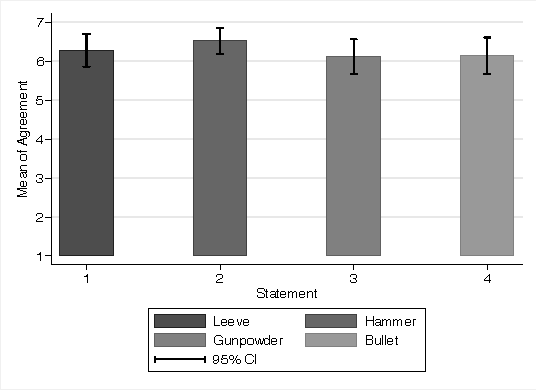
\includegraphics[scale=0.7]{figures/rev_com_bar.pdf}
      \caption{\textsf{\scriptsize(e) Simultaneous IOC, CRC, and CEQ Exclusion}}
      \label{fig:rev_com_bar}
   \end{subfigure}
   \caption{Means of agreements for the Replication (\ref{fig:rev_rep_bar}), the IOC Exclusion (\ref{fig:rev_ioc_bar}), the CRC Exclusion (\ref{fig:rev_crc_bar}), the CEQ Exclusion (\ref{fig:rev_ceq_bar}), as well as the Simultaneous IOC, CRC, and CEQ Exclusion (\ref{fig:rev_com_bar}) with the Revolver Vignette}\label{fig:rev}
\end{figure}
\end{landscape}

\begin{landscape}
\begin{table}[]
\resizebox{\linewidth}{!}{%
\begin{tabular}{lrlcccccccccc}
   \hline
                                  &                     &                                                                                                                                     &                         &           &                   &   & \multicolumn{3}{c}{Versus Neutral Value}       &   & \multicolumn{2}{c}{Versus Replication}   \\\cline{8-10}\cline{12-13} 
   Study                          &                     & Statement                                                                                                                           & $N$                     & $M$       & $95\%~CI$         &   & $z$        & $p$                  & $r$        &   & $z$        & $p$                         \\
   \hline\hline
   \multirow{4}{*}{Replication}   & \footnotesize (1)   & \footnotesize ``Leeve caused Uwe's death.''                                                                                         & \multirow{4}{*}{$63$}   & $6.603$   & $[6.285,6.922]$   &   & $ 7.108$   & $\leq 0.001^{***}$   & $ 0.896$   &   & $-$        & $-$                         \\
                                  & \footnotesize (2)   & \footnotesize ``The hammer caused Uwe's death.''                                                                                    &                         & $3.000$   & $[2.410,3.590]$   &   & $-3.288$   & $\leq 0.001^{***}$   & $-0.414$   &   & $-$        & $-$                         \\
                                  & \footnotesize (3)   & \footnotesize ``The gun powder caused Uwe's death.''                                                                                &                         & $2.984$   & $[2.402,3.566]$   &   & $-3.391$   & $\leq 0.001^{***}$   & $-0.427$   &   & $-$        & $-$                         \\
                                  & \footnotesize (4)   & \footnotesize ``The bullet caused Uwe's death.''                                                                                    &                         & $5.048$   & $[4.399,5.696]$   &   & $ 2.826$   & $0.005^{**}$         & $ 0.356$   &   & $-$        & $-$                         \\
   \hline
   \multirow{4}{*}{IOC}           & \footnotesize (1)   & \footnotesize ``Leeve's action of shooting at Uwe caused Uwe's death.''                                                             & \multirow{4}{*}{$54$}   & $5.648$   & $[5.062,6.234]$   &   & $ 4.404$   & $\leq 0.001^{***}$   & $ 0.599$   &   & $ 3.367$   & $\leq 0.001^{***}$          \\
                                  & \footnotesize (2)   & \footnotesize ``The release of the hammer caused Uwe's death.''                                                                     &                         & $3.667$   & $[2.988,4.346]$   &   & $-0.921$   & $0.357$              & $-0.125$   &   & $-1.754$   & $0.0795$                    \\
                                  & \footnotesize (3)   & \footnotesize ``The explosion of the gun powder caused Uwe's death.''                                                               &                         & $3.593$   & $[2.917,4.269]$   &   & $-1.230$   & $0.219$              & $-0.167$   &   & $-1.563$   & $0.1181$                    \\
                                  & \footnotesize (4)   & \footnotesize ``The bullet hitting Uwe caused Uwe's death.''                                                                        &                         & $6.241$   & $[5.770,6.712]$   &   & $ 5.766$   & $\leq 0.001^{***}$   & $ 0.785$   &   & $-2.767$   & $0.006^{**}$                \\
   \hline
   \multirow{4}{*}{CRC}           & \footnotesize (1)   & \footnotesize ``Uwe would not have died if Leeve had not shot at him.''                                                             & \multirow{4}{*}{$50$}   & $6.480$   & $[6.049,6.911]$   &   & $ 5.943$   & $\leq 0.001^{***}$   & $ 0.841$   &   & $ 0.410$   & $0.6819$                    \\
                                  & \footnotesize (2)   & \footnotesize\begin{tabular}[c]{@{}l@{}}``Uwe would not have died if the hammer\\ had not been released.''\end{tabular}             &                         & $6.120$   & $[5.582,6.658]$   &   & $ 5.339$   & $\leq 0.001^{***}$   & $ 0.755$   &   & $-6.615$   & $\leq 0.001^{***}$          \\
                                  & \footnotesize (3)   & \footnotesize\begin{tabular}[c]{@{}l@{}}``Uwe would not have died if the gun powder\\ had not exploded.''\end{tabular}              &                         & $5.720$   & $[5.110,6.330]$   &   & $ 4.463$   & $\leq 0.001^{***}$   & $ 0.631$   &   & $-5.855$   & $\leq 0.001^{***}$          \\
                                  & \footnotesize (4)   & \footnotesize ``Uwe would not have died if the bullet had not hit Uwe.''                                                            &                         & $6.160$   & $[5.633,6.687]$   &   & $ 5.165$   & $\leq 0.001^{***}$   & $ 0.730$   &   & $-2.505$   & $0.012$                     \\
   \hline
   \multirow{4}{*}{CEQ}           & \footnotesize (1)   & \footnotesize\begin{tabular}[c]{@{}l@{}}``Leeve's action of shooting at Uwe caused the release\\ of the hammer.''\end{tabular}      & \multirow{4}{*}{$53$}   & $4.962$   & $[4.270,5.654]$   &   & $ 2.565$   & $0.0103^{*}$         & $ 0.352$   &   & $ 4.399$   & $\leq 0.001^{***}$          \\
                                  & \footnotesize (2)   & \footnotesize\begin{tabular}[c]{@{}l@{}}``The release of the hammer caused the explosion\\ of the gun powder.''\end{tabular}        &                         & $5.830$   & $[5.272,6.389]$   &   & $ 4.911$   & $\leq 0.001^{***}$   & $ 0.675$   &   & $-6.015$   & $\leq 0.001^{***}$          \\
                                  & \footnotesize (3)   & \footnotesize ``The explosion of the gun powder caused the bullet to hit Uwe.''                                                     &                         & $5.056$   & $[4.396,5.717]$   &   & $ 2.943$   & $0.003^{**}$         & $ 0.404$   &   & $-4.471$   & $\leq 0.001^{***}$          \\
                                  & \footnotesize (4)   & \footnotesize ``The bullet hitting Uwe caused Uwe's death.''                                                                        &                         & $6.547$   & $[6.170,6.924]$   &   & $ 6.376$   & $\leq 0.001^{***}$   & $ 0.876$   &   & $-3.748$   & $\leq 0.001^{***}$          \\
   \hline
   \multirow{4}{*}{Combination}   & \footnotesize (1)   & \footnotesize\begin{tabular}[c]{@{}l@{}}``The hammer would not have released if Leeve\\ had not shot at Uwe.''\end{tabular}         & \multirow{4}{*}{$50$}   & $6.280$   & $[5.858,6.702]$   &   & $ 5.969$   & $\leq 0.001^{***}$   & $ 0.820$   &   & $ 1.682$   & $0.0926$                    \\
                                  & \footnotesize (2)   & \footnotesize\begin{tabular}[c]{@{}l@{}}``The gun powder would not have exploded if the hammer\\ had not released.''\end{tabular}   &                         & $6.520$   & $[6.194,6.846]$   &   & $ 6.232$   & $\leq 0.001^{***}$   & $ 0.856$   &   & $-7.377$   & $\leq 0.001^{***}$          \\
                                  & \footnotesize (3)   & \footnotesize\begin{tabular}[c]{@{}l@{}}``The bullet would not have hit Uwe if the gun powder\\ had not exploded.''\end{tabular}    &                         & $6.120$   & $[5.680,6.560]$   &   & $ 5.725$   & $\leq 0.001^{***}$   & $ 0.786$   &   & $-6.757$   & $\leq 0.001^{***}$          \\
                                  & \footnotesize (4)   & \footnotesize ``Uwe would not have died if the bullet had not hit Uwe.''                                                            &                         & $6.140$   & $[5.670,6.610]$   &   & $ 5.593$   & $\leq 0.001^{***}$   & $ 0.768$   &   & $-2.294$   & $0.0218$                    \\
   \hline\\[-1.5ex]
   \multicolumn{13}{p{26cm}}{\footnotesize\textit{$N$ gives the number of participants for each study. Thereafter, the mean agreement ($M$) and 95\% Confidence Intervals ($95\%~CI$) are given for every statement. Furthermore, the results of Wilcoxon signed-rank tests comparing the agreement to each statement with the neutral value of $4$ are reported, followed by the Effect Size ($r$), calculated by dividing the $z$ value by the square root of $N$. Additionally, two-sample Wilcoxon rank-sum tests are reported comparing the statements from subsequent studies to those from our replication. Asterisks denote significance levels: $^{*}p\le0.05$, $^{**}p\le0.01$, $^{***}p\le0.001$.}}
   \caption{Summary of Statements for the Revolver Vignette}\label{tab:rev_statements}
\end{tabular}}
\end{table}
\end{landscape}

\subsection{GFCI Vignette}\label{sec:results_cir}
Finally, a last set of studies was conducted with the GFCI Vignette:

\begin{quote}
   Mark is a scientist conducting a very important experiment on an unusual species of plant. His experiment requires growing his plants under a special light, which is plugged into an outlet with a Ground Fault Circuit Interrupter (GFCI) safety mechanism. The pipes running to Mark's laboratory were correctly manufactured and installed, and the system was protected from any changes in weather condition. Nonetheless, one day a pipe burst in Mark's laboratory. Water ran into the outlet powering the special light. A properly functioning GFCI is supposed to interrupt the circuit so that no power flows through its outlet. And indeed, the GFCI interrupted the circuit. The special light turned off and the experiment was ruined.
\end{quote}

\subsubsection{Replication}\label{sec:results_cir_rep}
As with the other vignettes, we tried to replicate the findings from L\&S (2020) first. Hence, subjects of our first study ($N=60$, male: $30$, female: $30$, mean age: $50.667$) had to rate the statements:

\begin{itemize}
   \item[(1)]\textsc{The pipe bursting caused the experiment to be ruined.}
   \item[(2)]\textsc{The GFCI breaking the circuit caused the experiment to be ruined.}
\end{itemize}

\noindent While the mean agreement of subjects from L\&S (2020, 63) was at $5.48$ and $3.67$, we obtained $5.483$ ($95\%~CI=[4.902,6.065]$) and $4.117$ ($95\%~CI=[6.285,6.922]$), as depicted in Figure \ref{fig:cir_rep_bar} (also see Figures \ref{fig:cir_rep_hist_1} and \ref{fig:cir_rep_hist_2} in Appendix \ref{app:additional_figures} for relative frequencies). Similar to the original data from L\&S (2020), Wilcoxon signed-rank tests show that the first statement is significantly different from the neutral value of $4$ ($p \leq 0.001$), the second one not so much, though ($z=0.403$, $p=0.687$). Hence, the findings from L\&S (2020) seem to be replicable with a German-speaking sample and a German translation of their vignette.

\subsubsection{Exclusion of the Intermediary-Ontology Confusion (IOC)}\label{sec:results_cir_ioc}
Trying to avoid the IOC by focussing on the events did not change the mean agreement with statement (2) much. Subjects ($N=64$, male: $38$, female: $26$, mean age: $50.000$) had to rate the two statements:

\begin{itemize}
   \item[(1)]\textsc{The pipe bursting caused the experiment to be ruined.}
   \item[(2)]\textsc{The breaking of the circuit by the GFCI caused the experiment to be ruined.}
\end{itemize}

\noindent Mean agreement with the second statement is at $4.234$ ($95\%~CI=[3.596,4.873]$), as can be seen in Figure \ref{fig:cir_ioc_bar} (also see Figures \ref{fig:cir_ioc_hist_1} and \ref{fig:cir_ioc_hist_2} in Appendix \ref{app:additional_figures} for relative frequencies). Again, a Wilcoxon signed-rank test indicates that the second statement is not different from the neutral value ($z=0.658$, $p=0.511$), showing practically no effect ($r=0.082$). That is, for the intermediary event, we see almost the same result as for the intermediary in the Poisoned Cup Vignette expressed by statement (2) and for the intermediaries in the Revolver Vignette expressed by the statements (2) and (3). Replacing individuals by events leads to a neutral response to the respective statements.

\subsubsection{Exclusion of the Causality-Responsibility Confusion (CRC)}\label{sec:results_cir_crc}
When we avoid the CRC by omitting talk of ``causation'', we obtain a result which is at first sight surprising compared to the other vignettes. Here, subjects ($N=67$, male: $37$, female: $30$, mean age: $46.267$) had to rate the statements:

\begin{itemize}
   \item[(1)]\textsc{The experiment would not have been ruined if the pipe had not burst.}
   \item[(2)]\textsc{The experiment would not have been ruined if the GFCI had not broken the circuit.}
\end{itemize}

\noindent The second statement was rated at $3.358$ ($95\%~CI=[2.720,3.996]$), as represented in Figure \ref{fig:cir_crc_bar} (also see Figures \ref{fig:cir_crc_hist_1} and \ref{fig:cir_crc_hist_2} in Appendix \ref{app:additional_figures} for relative frequencies). A Wilcoxon signed-rank tests shows that it is not significantly different from the scale's neutral value ($p=0.073$). The effect size is accordingly low ($r=0.254$). At first sight, this result might seem surprising. For the other vignettes, the CRC Exclusion led to highly significant agreements with the statements depicting intermediaries as causes. Now, the agreement with statement (2) even decreases compared to the second statements of the replication and the IOC Exclusion. However, the story of the GFCI Vignette makes the results plausible. Let us reconsider what happens in the vignette: The pipe burst, water ran into the outlet and made the GFCI break the circuit. What would have happened if there had been no GFCI installed in the circuit? The water in the outlet would have led to a short circuit, the special light would have turned off and the experiment would have been ruined nevertheless. We take this to be common sense knowledge. However, the GFCI safety mechanism reacts faster. Therefore, if there is a GFCI, then it breaks the circuit, but if there is no GFCI, the circuit breaks anyway. This means that we have a special case of \textit{preemption}, with the GFCI safety mechanism breaking the circuit being the preempting cause and the short circuit being the preempted cause. As is well known, preemption is a major challenge for the counterfactual theory of causation (\cite{lewis_causation_1973}): The breaking of the circuit by the GFCI causes the experiment to be ruined. However, subjects tend not to agree with statement (2) because the experiment would also have been ruined even if the GFCI had not broken the circuit (because of the short circuit). In light of this, we actually should have expected the results we obtained for the CRC Exclusion. In general: Confusing responsibility with causation because of the ambiguous meaning of the word ``cause'' cannot be ruled out by using counterfactual conditionals for cases including preemption.\footnote{We are aware of the fact that explaining our results with preemption is rather hypothetical at the moment. We think that more empirical research on preemption is required (for a brief overview see \citealt{henne_experimental_forthcoming}).} However, as we will see in the next section, the CEQ Exclusion alone is sufficient for doing so.

\subsubsection{Exclusion of the Cause-End Questioning (CEQ)}\label{sec:results_cir_ceq}
As for the other vignettes, we also constructed a causal chain to avoid the CEQ, using the statements:

\begin{itemize}
   \item[(1)]\textsc{The bursting of the pipe caused the GFCI to break to circuit.}
   \item[(2)]\textsc{The breaking of the circuit by the GFCI caused the special light to turn off.}
   \item[(3)]\textsc{The special light turning off caused the experiment to be ruined.}
\end{itemize}

\noindent In this case, subjects ($N=64$, male: $29$, female: $35$, mean age: $47.516$) evaluated the second statement at $6.250$ ($95\%~CI=[5.835,6.665]$), as can be seen in Figure \ref{fig:cir_ceq_bar} (also see Figures \ref{fig:cir_ceq_hist_1}, \ref{fig:cir_ceq_hist_2}, and \ref{fig:cir_ceq_hist_3} in Appendix \ref{app:additional_figures} for relative frequencies). A Wilcoxon signed-rank test shows that this evaluation is significantly different from the neutral value ($p \leq 0.001$); with a large effect ($r=0.790$). Compared to the disagreements with statement (2) of the replication, subjects now strongly agree that the breaking of the circuit by the GFCI is a cause in the causal chain that in the end leads to a ruined experiment. The reason for this is that subjects do not consider the responsibility of the intermediary for the end link of the causal chain because of the CEQ Exclusion. The CEQ, as applied by L\&S (2020), supports the CRC and, thus, leads subjects to consider the responsibility of the intermediary for the ruined experiment. Thus, excluding the CEQ shows a clear effect in support of the CCAC.

\subsubsection{Simultaneous IOC, CRC, and CEQ Exclusion}\label{sec:results_cir_com}
Lastly, a combination of the variations above introduced consisted of the statements:

\begin{itemize}
   \item[(1)]\textsc{The GFCI would not have broken the circuit if the pipe had not burst.}
   \item[(2)]\textsc{The special light would not have turned off if the GFCI had not broken the circuit.}
   \item[(3)]\textsc{The experiment would not have been ruined if the special light had not turned off.}
\end{itemize}

\noindent Similar to the causal chain in Section \ref{sec:results_cir_ceq}, subjects ($N=59$, male: $38$, female: $21$, mean age: $51.356$) evaluated statement (2) at $6.186$ ($95\%~CI=[5.734,6.639]$), as can be seen in Figure \ref{fig:cir_com_bar} (also see Figures \ref{fig:cir_com_hist_1}, \ref{fig:cir_com_hist_2}, and \ref{fig:cir_com_hist_3} in Appendix \ref{app:additional_figures} for relative frequencies). A Wilcoxon signed-rank tests shows that, again, it is significantly different from $4$ ($p \leq 0.001$), with a large effect ($r=0.775$). Again, we found a very high agreement for the GFCI safety mechanism breaking the circuit being a cause in the causal chain, contrary to the results of L\&S (2020). Apparently, the modifications IOC Exclusion and CRC Exclusion, which both do not lead to an agreement with the respective second statements independently, are overruled by the CEQ Exclusion. In sum, the simultaneous exclusion of IOC, CRC, and CEQ strongly supports the CCAC, contrary to L\&S (2020).

\subsubsection{Summary}\label{sec:results_cir_sum}
Figure \ref{fig:cir} shows the means of our subjects' agreements to the respective statements for the Replication (Figure \ref{fig:cir_rep_bar}), the IOC Exclusion (Figure \ref{fig:cir_ioc_bar}), the CRC Exclusion (Figure \ref{fig:cir_crc_bar}), the CEQ Exclusion (Figure \ref{fig:cir_ceq_bar}), as well as the Simultaneous IOC, CRC, and CEQ Exclusion (Figure \ref{fig:cir_com_bar}). Additionally, Table \ref{tab:cir_statements} summarizes the statements presented in our studies on the GFCI Vignette. For the CEQ Exclusion as well as the simultaneous IOC, CRC, and CEQ Exclusion, we found highly significant agreements with the respective second statements, evaluated significantly different from our replication. However, we found an interesting pattern for the CRC Exclusion diverging from our results of the Poisoned Cup Vignette and the Revolver Vignette which, as we hypothesize, results from the GFCI Vignette involving a case of preemption. Hence, testing the concept of causation by counterfactual conditionals should have been expected to fail for this vignette. Nevertheless, the CEQ Exclusion alone leads to strong evidence supporting the CCAC for the same vignette as used by L\&S.

\begin{landscape}
\begin{figure}[h!]
   \begin{subfigure}[t]{0.28\textwidth}
      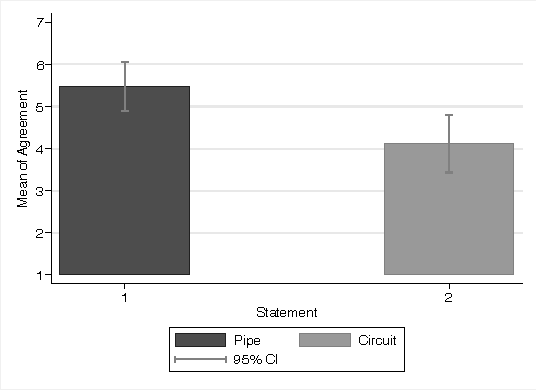
\includegraphics[scale=0.7]{figures/cir_rep_bar.pdf}
      \caption{\textsf{\scriptsize(a) Replication}}
      \label{fig:cir_rep_bar}
   \end{subfigure}
   \begin{subfigure}[t]{0.28\textwidth}
      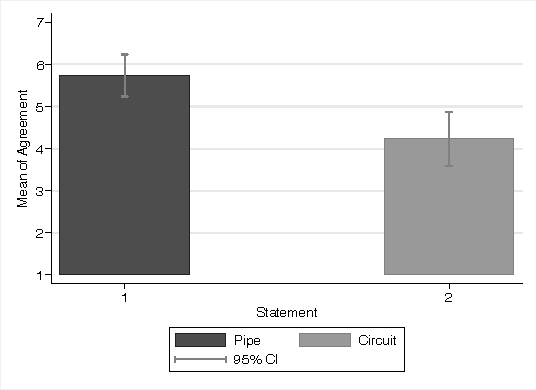
\includegraphics[scale=0.7]{figures/cir_ioc_bar.pdf}
      \caption{\textsf{\scriptsize(b) IOC Exclusion}}
      \label{fig:cir_ioc_bar}
   \end{subfigure}
   \begin{subfigure}[t]{0.28\textwidth}
      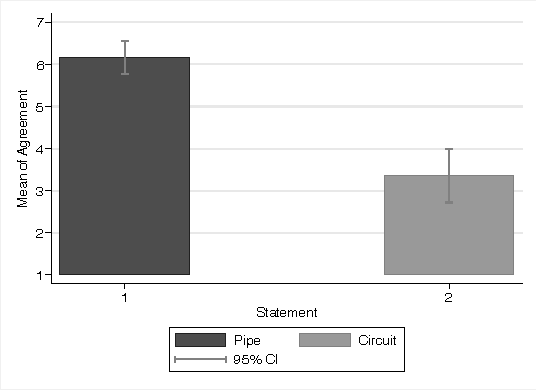
\includegraphics[scale=0.7]{figures/cir_crc_bar.pdf}
      \caption{\textsf{\scriptsize(c) CRC Exclusion}}
      \label{fig:cir_crc_bar}
   \end{subfigure}
   \begin{subfigure}[t]{0.28\textwidth}
      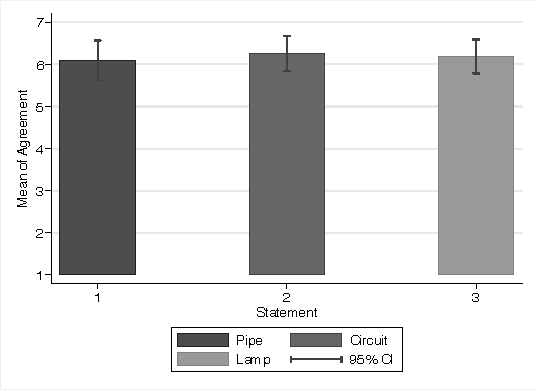
\includegraphics[scale=0.7]{figures/cir_ceq_bar.pdf}
      \caption{\textsf{\scriptsize(d) CEQ Exclusion}}
      \label{fig:cir_ceq_bar}
   \end{subfigure}
   \begin{subfigure}[t]{0.28\textwidth}
      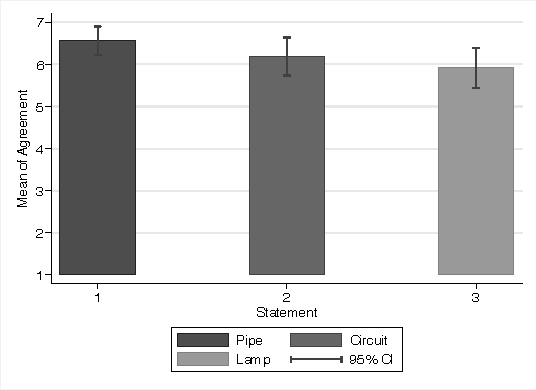
\includegraphics[scale=0.7]{figures/cir_com_bar.pdf}
      \caption{\textsf{\scriptsize(e) Simultaneous IOC, CRC, and CEQ Exclusion}}
      \label{fig:cir_com_bar}
   \end{subfigure}
   \caption{Means of agreements for the Replication (\ref{fig:cir_rep_bar}), the IOC Exclusion (\ref{fig:cir_ioc_bar}), the CRC Exclusion (\ref{fig:cir_crc_bar}), the CEQ Exclusion (\ref{fig:cir_ceq_bar}), as well as the Simultaneous IOC, CRC, and CEQ Exclusion (\ref{fig:cir_com_bar}) with the GFCI Vignette}\label{fig:cir}
\end{figure}
\end{landscape}

\begin{landscape}
\begin{table}[]
\resizebox{\linewidth}{!}{%
\begin{tabular}{lrlcccccccccc}
   \hline
                                  &                     &                                                                                                                                                  &                         &           &                   &   & \multicolumn{3}{c}{Versus Neutral Value}       &   & \multicolumn{2}{c}{Versus Replication}   \\\cline{8-10}\cline{12-13}
   Study                          &                     & Statement                                                                                                                                        & $N$                     & $M$       & $95\%~CI$         &   & $z$        & $p$                  & $r$        &   & $z$        & $p$                         \\
   \hline\hline
   \multirow{2}{*}{Replication}   & \footnotesize (1)   & \footnotesize ``The pipe bursting caused the experiment to be ruined.''                                                                          & \multirow{2}{*}{$60$}   & $5.483$   & $[4.902,6.065]$   &   & $ 4.369$   & $\leq 0.001^{***}$   & $ 0.564$   &   & $-$        & $-$                         \\
                                  & \footnotesize (2)   & \footnotesize\begin{tabular}[c]{@{}l@{}}``The GFCI breaking the circuit\\ caused the experiment to be ruined.''\end{tabular}                     &                         & $4.117$   & $[3.434,4.799]$   &   & $ 0.403$   & $0.6871$             & $ 0.052$   &   & $-$        & $-$                         \\
   \hline
   \multirow{2}{*}{IOC}           & \footnotesize (1)   & \footnotesize ``The pipe bursting caused the experiment to be ruined.''                                                                          & \multirow{2}{*}{$64$}   & $5.734$   & $[5.236,6.232]$   &   & $ 5.310$   & $\leq 0.001^{***}$   & $ 0.664$   &   & $-0.556$   & $0.5781$                    \\
                                  & \footnotesize (2)   & \footnotesize\begin{tabular}[c]{@{}l@{}}``The breaking of the circuit by the GFCI caused\\ the experiment to be ruined.''\end{tabular}           &                         & $4.234$   & $[3.596,4.873]$   &   & $ 0.658$   & $0.511$              & $ 0.082$   &   & $-0.122$   & $0.9028$                    \\
   \hline
   \multirow{2}{*}{CRC}           & \footnotesize (1)   & \footnotesize\begin{tabular}[c]{@{}l@{}}``The experiment would not have been ruined if\\ the pipe had not burst.''\end{tabular}                  & \multirow{2}{*}{$67$}   & $6.164$   & $[5.771,6.557]$   &   & $ 6.484$   & $\leq 0.001^{***}$   & $ 0.917$   &   & $-1.760$   & $0.0785$                    \\
                                  & \footnotesize (2)   & \footnotesize\begin{tabular}[c]{@{}l@{}}``The experiment would not have been ruined if\\ the GFCI had not broken the circuit.''\end{tabular}     &                         & $3.358$   & $[2.720,3.996]$   &   & $-1.794$   & $0.0728$             & $ 0.254$   &   & $ 1.566$   & $0.1173$                    \\
   \hline
   \multirow{3}{*}{CEQ}           & \footnotesize (1)   & \footnotesize\begin{tabular}[c]{@{}l@{}}``The bursting of the pipe caused the\\ GFCI to break to circuit.''\end{tabular}                         & \multirow{3}{*}{$64$}   & $6.094$   & $[5.619,6.568]$   &   & $ 6.039$   & $\leq 0.001^{***}$   & $ 0.755$   &   & $-2.155$   & $ 0.0312$                   \\
                                  & \footnotesize (2)   & \footnotesize\begin{tabular}[c]{@{}l@{}}``The breaking of the circuit by the\\ GFCI caused the special light to turn off.''\end{tabular}         &                         & $6.250$   & $[5.834,6.665]$   &   & $ 6.317$   & $\leq 0.001^{***}$   & $ 0.790$   &   & $-4.842$   & $\leq 0.001^{***}$          \\
                                  & \footnotesize (3)   & \footnotesize\begin{tabular}[c]{@{}l@{}}``The special light turning off caused the experiment to be ruined.''\end{tabular}                       &                         & $6.188$   & $[5.785,6.590]$   &   & $ 6.628$   & $\leq 0.001^{***}$   & $ 0.828$   &   & $-$        & $-$                         \\
   \hline
   \multirow{3}{*}{Combination}   & \footnotesize (1)   & \footnotesize\begin{tabular}[c]{@{}l@{}}``The GFCI would not have\\ broken the circuit if the pipe had not burst.''\end{tabular}                 & \multirow{3}{*}{$59$}   & $6.559$   & $[6.220,6.899]$   &   & $ 6.780$   & $\leq 0.001^{***}$   & $ 0.883$   &   & $-3.391$   & $\leq 0.001^{***}$          \\
                                  & \footnotesize (2)   & \footnotesize\begin{tabular}[c]{@{}l@{}}``The special light would not have turned off if\\ the GFCI had not broken the circuit.''\end{tabular}   &                         & $6.186$   & $[5.734,6.639]$   &   & $ 5.949$   & $\leq 0.001^{***}$   & $ 0.775$   &   & $-4.619$   & $\leq 0.001^{***}$          \\
                                  & \footnotesize (3)   & \footnotesize\begin{tabular}[c]{@{}l@{}}``The experiment would not have been ruined if\\ the special light had not turned off.''\end{tabular}    &                         & $5.915$   & $[5.438,6.393]$   &   & $ 5.508$   & $\leq 0.001^{***}$   & $ 0.717$   &   & $-$        & $-$                         \\
   \hline\\[-1.5ex]
   \multicolumn{13}{p{26cm}}{\footnotesize\textit{$N$ gives the number of participants for each study. Thereafter, the mean agreement ($M$) and 95\% Confidence Intervals ($95\%~CI$) are given for every statement. Furthermore, the results of Wilcoxon signed-rank tests comparing the agreement to each statement with the neutral value of $4$ are reported, followed by the Effect Size ($r$), calculated by dividing the $z$ value by the square root of $N$. Additionally, two-sample Wilcoxon rank-sum tests are reported comparing the statements from subsequent studies to those from our replication. Asterisks denote significance levels: $^{*}p\le0.05$, $^{**}p\le0.01$, $^{***}p\le0.001$.}}
   \caption{Summary of Statements for the GFCI Vignette}\label{tab:cir_statements}
\end{tabular}}
\end{table}
\end{landscape}

\section{Conclusion}\label{sec:conclusion}
In this article, we argue that the results of L\&S (2020) are caused by three interrelated problems: The Intermediary-Ontology Confusion (IOC), the Causality-Responsibility Confusion (CRC), and the Cause-End Questioning (CEQ). The design of L\&S (2020) suffers from all of them. Hence, it generates effects leading subjects to confuse causality with responsibility. We hypothesized that excluding the IOC, the CRC, and the CEQ would lead to results supporting the Compositionality Constraint of Actual Causation (CCAC) for the same vignettes originally used by L\&S (2020) to challenge the CCAC.

In order to investigate this assumption, we replicated the results of L\&S (2020) and successively tested modifications that aimed at excluding the IOC, the CRC, and the CEQ. In a last step, we tested all modifications simultaneously. Our results focus on the intermediaries of the causal chains presented in the vignettes because the results of L\&S (2020) seemed to show primarily that laypeople tend to disagree that the intermediaries of the causal chains are causes.

Excluding the IOC, according to our studies, leads to less disagreement that the intermediaries are causes for all vignettes. We assume that the reason for this is that replacing individuals by events reduces responsibility considerations triggered by individuals. For the Poisoned Cup Vignette, L\&S (2020) obtained similar results. Hence, we expected our findings to apply to all three vignettes.

Excluding the CRC leads to strong evidence that -- contrary to the results of L\&S (2020) -- intermediaries are conceived to be causes for the Poisoned Cup Vignette and the Revolver Vignette. Asking about the concept of causation without using the ambiguous word ``causation'' prevents subjects from confusing causality with responsibility. The modification CRC Exclusion does not work for the GFCI Vignette. In hindsight, the reason for this seems to be obvious: The GFCI Vignette contains a case of preemption and counterfactual conditionals should be expected not to work for cases of preemption because preemption is a major problem for the counterfactual theory of causation. However, we leave this question open for future research in the experimental philosophy of causation.

Excluding the CEQ strongly supports our hypothesis that intermediaries that are presented as direct causes of the undesirable and awful end links of the chains trigger the confusion of causality and responsibility. If an intermediary $d_{1}$ is presented as a cause of a further intermediary $d_{2}$, then $d_{1}$ is not judged to be something which is responsible for an awful event but perceived as a cause in a chain of causes and effects. Hence, excluding the CEQ leads to a high agreement that intermediaries are causes, contrary to the findings of L\&S (2020).

Excluding the IOC, the CRC, and the CEQ simultaneously leads to a highly significant agreement that the intermediaries of the replications are causes for all vignettes. The effect sizes for the respective statements are in all cases high or very high. That means that the same intermediaries that were all assessed \textit{not} to be causes in L\&S (2020) are now assessed to \textit{be} causes. We take this to be strong evidence in support of the CCAC.

Lastly, we think that our results challenge the RV, which takes \textit{responsibility} to be part of the concept \textit{causation}. However, this point is not subject of this article and -- as does the problem of preemption -- deserves further investigation.


\section{Acknowledgements}
We are thankful to Mark Siebel, Ewgenia Baraboj, Jonathan Livengood, and Justin Sytsma.   


\clearpage
\printbibliography

\clearpage
\section*{Appendix}
\appendix
\section{Pilot Studies}\label{app:pilot}
We limited the pilot to the Poisoned Cup Vignette. First, subjects were greeted with a welcome message:

\begin{quote}
   Welcome to our study!%Herzlich willkommen zu unserer Studie!
	
   If you focus on the task, you will probably need no more than five to ten minutes for this study. It is important that you read the instructions carefully. Also, please complete the study without closing your browser in between.%Bei konzentrierter Bearbeitung werden Sie voraussichtlich nicht länger als fünf bis zehn Minuten für diese Studie benötigen. Es ist wichtig, dass Sie die Hinweise und Aufgaben aufmerksam lesen. Bearbeiten Sie die Studie bitte außerdem, ohne den Browser zwischendurch zu schließen.

   We will evaluate your assessment as well as the assessments of all other participants in this study. All data will be stored in anonymized form so that no information can be assigned to an individual person. The results of the study will be published.%Wir werden Ihre Einschätzungen sowie die Einschätzungen aller anderen Teilnehmerinnen und Teilnehmer dieser Studie auswerten. Alle Daten werden in anonymisierter Form gespeichert, so dass keine Angaben einer einzelnen Person zugeordnet werden können. Die Ergebnisse der Studie werden veröffentlicht.

   Thank you for your participation!%Vielen Dank für Ihre Teilnahme!
\end{quote}

Thereafter, they were introduced to the vignette that we adapted from L\&S (2020):

\begin{quote}
   Gabi wants to kill her daughter, Nele, but she doesn't want to go to prison for murder. As such, Gabi hatches a plan. She arranges for a baby sitter, Kathrin, to take care of Nele while she herself is out of town on business. Before leaving, Gabi laces one of Nele's sippy cups with a deadly poison that is very difficult to detect. That evening, Kathrin gives Nele juice in the poisoned sippy cup. Nele drinks the juice and dies two hours later.%Gabi will ihre Tochter Nele töten, aber sie will nicht wegen Mordes ins Gefängnis gehen. Deshalb heckt Gabi einen Plan aus. Sie engagiert eine Babysitterin, Kathrin, die sich um Nele kümmert, während Gabi geschäftlich unterwegs ist. Bevor Gabi geht, versieht sie einen von Neles Trinkbechern mit einem tödlichen Gift, das sehr schwer nachzuweisen ist. An demselben Abend gibt Kathrin Nele Saft mit dem vergifteten Trinkbecher. Nele trinkt den Saft und stirbt zwei Stunden später.
\end{quote}

\noindent Subsequently, subjects were asked to state their disagreement or agreement with several statements about the vignette on a scale from $1$ (``don't agree at all'') to $7$ (``totally agree''). In total, eight pilot studies were conducted. Studies 1 and 2 were replications of two studies from L\&S (2020). While Study 1 asked about the causal role of Gabi and Kathrin, Study 2 asked about the causal role of their actions. Study 3, then, varied the wording used in Study 2, omitting the names of Gabi and Kathrin, in order to place special emphasis on the actions, not the agents. Studies 4 and 5, on the other hand, avoided the mention of ``causation''. Instead, Study 4 asked whether Nele would have died, too, if the actions of Gabi or Kathrin had not happened. In a different manner, Study 5 asked whether Nele died because of the actions of Gabi or Kathrin. Study 6 then introduced a causal chain, with Gabi giving the poisoned cup to Kathrin, Kathrin giving it to Nele, and Nele drinking from it. Lastly, Studies 7 and 8 combined the approach from Study 6 with those from Studies 4 and 5. Each study consisted of two or three statements that were displayed to subjects on the same screen and in a fixed order as follows:

\begin{description}
   \item [Study 1:] (1) Gabi caused Neles death. (2) Kathrin caused Neles death.% (1) Gabi verursachte Neles Tod. (2) Kathrin verursachte Neles Tod.
   \item [Study 2:] (1) Gabi's action of poisoning the sippy cup caused Nele's death. (2) Kathrin's action of giving Nele juice with a sippy cup that was poisoned caused Nele's death.% (1) Gabis Handlung, den Trinkbecher zu vergiften, verursachte Neles Tod. (2) Kathrins Handlung, Nele Saft mit einem Trinkbecher zu geben, der vergiftet war, verursachte Neles Tod.
   \item [Study 3:] (1) The action of poisoning the sippy cup caused Nele's death. (2) The action of giving Nele juice with a sippy cup that was poisoned caused Nele's death.% (1) Die Handlung, den Trinkbecher zu vergiften, verursachte Neles Tod. (2) Die Handlung, Nele Saft mit einem Trinkbecher zu geben, der vergiftet war, verursachte Neles Tod.
   \item [Study 4:] (1) Nele would have died that night, too, if Gabi hadn't poisoned the sippy cup. (2) Nele would have died that night, too, if Kathrin had given her juice with a sippy cup that wasn't poisoned.% (1) Nele wäre an dem Abend auch gestorben, wenn Gabi den Trinkbecher nicht vergiftet hätte. (2) Nele wäre an dem Abend auch gestorben, wenn Kathrin ihr Saft mit einem Trinkbecher gegeben hätte, der nicht vergiftet war.
   \item [Study 5:] (1) Nele died that night because Gabi poisoned the sippy cup. (2) Nele died that night because Kathrin gave her juice with a sippy cup that was poisoned.% (1) Nele ist an dem Abend gestorben, weil Gabi den Trinkbecher vergiftet hat. (2) Nele ist an dem Abend gestorben, weil Kathrin ihr Saft mit einem Trinkbecher gegeben hat, der vergiftet war.
   \item [Study 6:] (1) Gabi poisoning Nele's sippy cup caused Kathrin to give Nele juice with a sippy cup that was poisoned. (2) Kathrin giving Nele juice with a sippy cup that was poisoned caused Nele to ingest poison. (3) Nele ingesting poison caused Nele to die.% (1) Dass Gabi Neles Trinkbecher mit Gift versehen hat, verursachte, dass Kathrin Nele Saft mit einem Trinkbecher gegeben hat, der vergiftet war. (2) Dass Kathrin Nele Saft mit einem Trinkbecher gegeben hat, der vergiftet war, verursachte, dass Nele Gift zu sich genommen hat. (3) Dass Nele Gift zu sich nahm, verursachte, dass Nele starb.
   \item [Study 7:] (1) Kathrin would have given Nele juice with a sippy cup that was poisoned even if Gabi hadn't poisoned Nele's sippy cup. (2) Nele would also have ingested poison if Kathrin had given her juice with a sippy cup that was not poisoned. (3) Nele would also have died if she had not ingested the poison.% (1) Kathrin hätte Nele auch dann Saft mit einem Trinkbecher gegeben, der vergiftet war, wenn Gabi Neles Trinkbecher nicht mit Gift versehen hätte. (2) Nele hätte auch Gift zu sich genommen, wenn Kathrin ihr Saft mit einem Trinkbecher gegeben hätte, der nicht vergiftet war. (3) Nele wäre auch gestorben, wenn sie das Gift nicht zu sich genommen hätte.
   \item [Study 8:] (1) Kathrin gave Nele juice with a sippy cup that was poisoned because Gabi had poisoned Nele's sippy cup. (2) Nele ingested poison because Kathrin gave Nele juice with a sippy cup that was poisoned. (3) Nele died because she ingested poison.% (1) Kathrin hat Nele Saft mit einem Trinkbecher gegeben, der vergiftet war, weil Gabi Neles Trinkbecher mit Gift versehen hatte. (2) Nele hat Gift zu sich genommen, weil Kathrin Nele Saft mit einem Trinkbecher gegeben hat, der vergiftet war. (3) Nele starb, weil sie Gift zu sich genommen hat.
\end{description}

\noindent The pilot studies were programmed in \citet{limesurvey_limesurvey_2021} and conducted online in February 2021. Subjects were recruited by the private market research institute \textit{respondi}, where they were randomly drawn from a pool of registered users from Germany. All texts were presented to them in German. Two control questions were asked to ensure that subjects have read the vignettes and instructions carefully.\footnote{The first read: ``Did Kathrin poison Nele's sippy cup?'' The second: ``Did Gabi give the poisoned sippy cup to Nele?'' Both had a binary answering option (``yes'' or ``no''). They were displayed to subjects on two separate screens right after they had completed the main task.
%Hat Kathrin Neles Trinkbecher vergiftet? Hat Gabi Nele den vergifteten Trinkbecher gegeben?
A total of $121$ subjects dropped out of the pilot studies because they failed to answer both control questions correctly. As had been declared beforehand by \textit{respondi}, they were not compensated.} We limited our analysis to those subjects who passed both questions correctly. Those subjects were paid a flat fee of $2.10$ euro, equivalent to an hourly wage of $12.60$ euro.

The total sample size of our pilot studies was $N=164$. $81$ ($49.39\%$) of our subjects stated to be female, another $83$ ($50.61\%$) stated to be male. The mean of their age was $44.47$ years.

In Study 1 (see Figure \ref{fig:pilot_study_1}), the mean agreement with Statement (1) is at $6.176$ ($95\%$ $CI=[5.144,7.209]$), while the agreement with Statement (2) is only at $2.118$ ($95\%~CI=[1.044,3.191]$) ($N=17$, male: $5$, female: $12$, mean age: $48.00$). This is very close to the results from L\&S (2020, 50), since the reported mean for their Statement (1) was at $7.00$ and for their Statement (2) at $2.06$.

\begin{figure}[H]
   \centering
   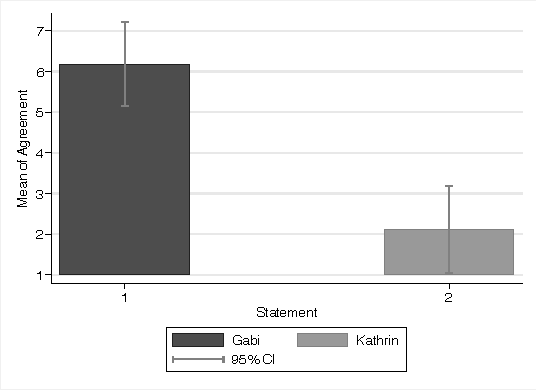
\includegraphics[scale=0.8]{figures/pilot_study_1.pdf}
   \begin{minipage}{0.9\linewidth}
   \footnotesize
   \emph{The figure shows the mean of subjects' agreements with the statements ``Gabi caused Neles death'' and ``Kathrin caused Neles death''. $N=17$.}
   \end{minipage}
   \caption{Mean of agreements in Pilot Study 1}
   \label{fig:pilot_study_1}
\end{figure}

\noindent Study 2 shows a similiar picture (see Figure \ref{fig:pilot_study_2}). Here, the mean agreement with Statement (1) is similarly high at $6.231$ ($95\%~CI=[5.505,6.956]$), while the mean agreement with Statement (2) is slightly higher than in Study 1 at $3.423$ ($95\%~CI=[2.356,4.490]$) ($n=26$, male: $15$, female: $11$, mean age: $47.35$). Again, results are very close to those from L\&S (2020, 55). The reported mean for their Statement (1) was at $6.52$ and for their Statement (2) at $3.36$.

\begin{figure}[H]
   \centering
   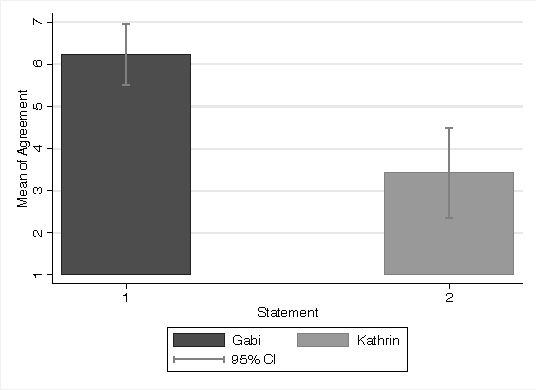
\includegraphics[scale=0.8]{figures/pilot_study_2.pdf}
   \begin{minipage}{0.9\linewidth}
   \footnotesize
   \emph{The figure shows the mean of subjects' agreements with the statements ``Gabi's action of poisoning the sippy cup caused Nele's death'' and ``Kathrin's action of giving Nele juice with a sippy cup that was poisoned caused Nele's death''. $N=26$.}
   \end{minipage}
   \caption{Mean of agreements in Pilot Study 2}
   \label{fig:pilot_study_2}
\end{figure}

\noindent Omitting the names of Gabi and Kathrin in Study 3 (see Figure \ref{fig:pilot_pilot_3}) resulted in some slightly changed means. In this case, the mean agreement with Statement (1) is slightly lower at $5.300$ ($95\%~CI=[4.084,6.516]$), while the mean agreement with Statement (2) is slightly higher at $4.200$ ($95\%~CI=[2.952,5.448]$) ($N=20$, male: $10$, female: $10$, mean age: $43.00$). Although statistical analysis on sample sizes that small is problematic, two Wilcoxon rank-sum tests indicate that the null-hypotheses of equal means between Studies 2 and 3 cannot be rejected neither for Statement (1) ($z=1.635$, $p=0.102$) nor for Statement (2) ($z=0.854$, $p=0.393$).

\begin{figure}[H]
   \centering
   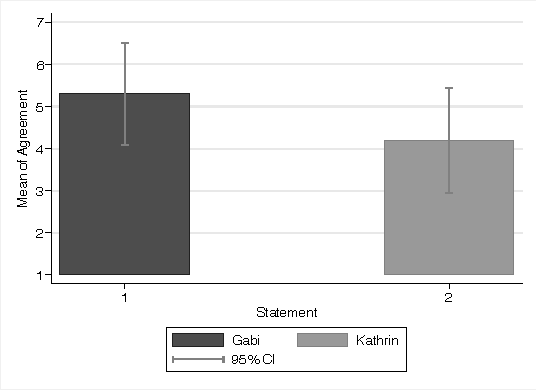
\includegraphics[scale=0.8]{figures/pilot_study_3.pdf}
   \begin{minipage}{0.9\linewidth}
   \footnotesize
   \emph{The figure shows the mean of subjects' agreements with the statements ``The action of poisoning the sippy cup caused Nele's death'' and ``The action of giving Nele juice with a sippy cup that was poisoned caused Nele's death''. $N=20$.}
   \end{minipage}
   \caption{Mean of agreements in Pilot Study 3}
   \label{fig:pilot_pilot_3}
\end{figure}

\noindent Avoiding the mention of ``causation'' and presenting the statements in a counterfactual phrasing in Study 4 (see Figure \ref{fig:pilot_study_4}) resulted in strikingly equal (dis)agreements with Statements (1) and (2). Since their phrasing reframed the scale (now \textit{low} agreements indicate a \textit{high} causal relevance, as they suggest that the effect would not have occurred without the action in question), we recoded the answers (the scale was coded in reversed order) for better comparability. The mean of (recoded) agreements with Statement (1) is at $6.357$ ($95\%~CI=[5.407,7.307]$), with a similar mean of (recoded) agreements with Statement (2) at $6.571$ ($95\%~CI=[5.796,7.347]$) ($N=14$, male: $7$, female: $7$, mean age: $39.79$).

\begin{figure}[H]
   \centering
   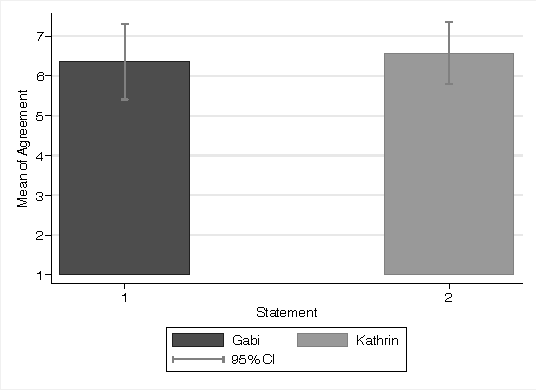
\includegraphics[scale=0.8]{figures/pilot_study_4.pdf}
   \begin{minipage}{0.9\linewidth}
   \footnotesize
   \emph{The figure shows the mean of subjects' (recoded) agreements with the statements ``Nele would have died that night, too, if Gabi hadn't poisoned the sippy cup'' and ``Nele would have died that night, too, if Kathrin had given her juice with a sippy cup that wasn't poisoned''. Values were recoded in reversed order for better comparability. $N=14$.}
   \end{minipage}
   \caption{Mean of agreements in Pilot Study 4 (recoded in reversed order)}
   \label{fig:pilot_study_4}
\end{figure}

\noindent Changing the phrasing in Study 5 (see Figure \ref{fig:pilot_study_5}) resulted in a similar pattern. Here, mention of ``causation'' is still avoided, while the statements are phrased as giving reasons with ``because''. This time, the mean agreement with Statement (1) is at $5.480$ ($95\%~CI=[4.413,6.547]$) and the mean agreement with Statement (2) similarly high at $5.28$ ($95\%~CI=[4.272,6.288]$) ($N=25$, male: $15$, female: $10$, mean age: $42.76$). Again, two Wilcoxon rank-sum tests indicate that the null-hypotheses of equal means between Studies 4 and 5 cannot be rejected neither for Statement (1) ($z=1.339$, $p=0.181$) nor for Statement (2) ($z=1.775$, $p=0.076$), given that we use the recoded data for Study~4.

\begin{figure}[H]
   \centering
   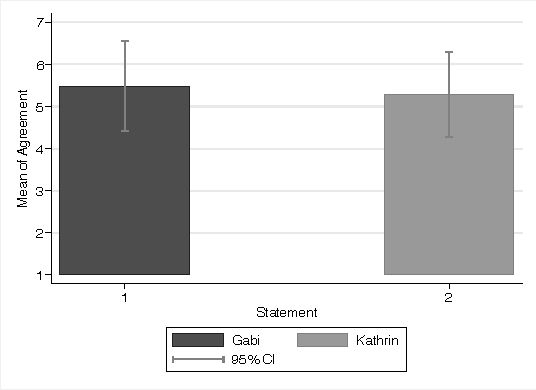
\includegraphics[scale=0.8]{figures/pilot_study_5.pdf}
   \begin{minipage}{0.9\linewidth}
   \footnotesize
   \emph{The figure shows the mean of subjects' agreements with the statements ``Nele died that night because Gabi poisoned the sippy cup'' and ``Nele died that night because Kathrin gave her juice with a sippy cup that was poisoned''. $N=14$.}
   \end{minipage}
   \caption{Mean of agreements in Pilot Study 5}
   \label{fig:pilot_study_5}
\end{figure}

\noindent When presented as a chain of events in Study 6 (see Figure \ref{fig:pilot_study_6}), the causal role of each element for the next in line is evaluated constantly high. Here, the mean agreement with Statement (1) is at $5.850$ ($95\%~CI=[4.784,6.916]$), the mean agreement with Statement (2) at $5.400$ ($95\%~CI=[4.260,6.540]$), and the mean agreement with Statement (3) at $6.300$ ($95\%~CI=[5.440,7.160]$) ($N=20$, male: $11$, female: $9$, mean age: $40.70$).

\begin{figure}[H]
   \centering
   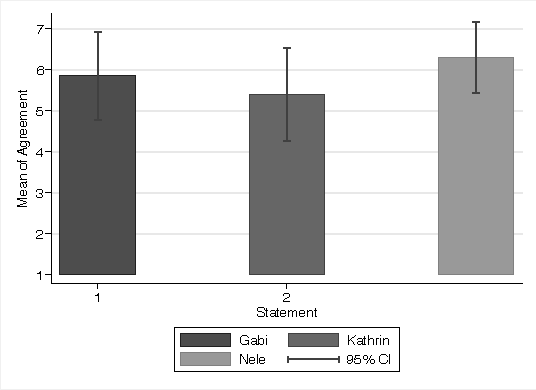
\includegraphics[scale=0.8]{figures/pilot_study_6.pdf}
   \begin{minipage}{0.9\linewidth}
   \footnotesize
   \emph{The figure shows the mean for agreements with the statements ``Gabi poisoning Nele's sippy cup caused Kathrin to give Nele juice with a sippy cup that was poisoned'', ``Kathrin giving Nele juice with a sippy cup that was poisoned caused Nele to ingest poison'', and ``Nele ingesting poison caused Nele to die''. $N=20$.}
   \end{minipage}
   \caption{Mean of agreements in Pilot Study 6}
   \label{fig:pilot_study_6}
\end{figure}

\noindent Combining the approaches from Study 4 and 6 in Study 7 (see Figure \ref{fig:pilot_study_7}) results in a similar picture. As for Study 4, answers were recoded in reversed order for better comparability. Here, the mean of (recoded) agreements with Statement (1) is slightly lower at $4.476$ ($95\%~CI=[3.152,5.800]$), the mean of (recoded) agreement with Statement (2) is at $6.762$ ($95\%~CI=[6.443,7.081]$), and the mean of (recoded) agreement with Statement (3) is at $6.190$ ($95\%~CI=[5.448,6.933]$) ($N=21$, male: $10$, female: $11$, mean age: $45.71$).

\begin{figure}[H]
   \centering
   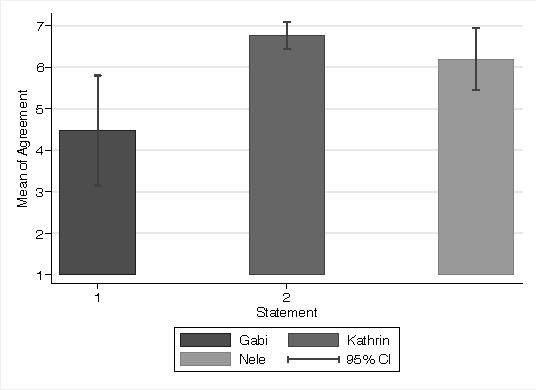
\includegraphics[scale=0.8]{figures/pilot_study_7.pdf}
   \begin{minipage}{0.9\linewidth}
   \footnotesize
   \emph{The figure shows the mean of (recoded) agreements with the statements ``Kathrin would have given Nele juice with a sippy cup that was poisoned even if Gabi hadn't poisoned Nele's sippy cup'', ``Nele would also have ingested poison if Kathrin had given her juice with a sippy cup that was not poisoned'', and ``Nele would also have died if she had not ingested the poison''. Values were recoded in reversed order for better comparability. $N=21$.}
   \end{minipage}
   \caption{Mean of agreements in Pilot Study 7 (recoded in reversed order)}
   \label{fig:pilot_study_7}
\end{figure}

\noindent Lastly, combining the approaches from Study 5 and 6 in Study 8 (see Figure \ref{fig:pilot_study_8}), again produces a similar picture. The mean agreement with Statement (1) is at $5.905$ ($95\%~CI=[4.919,6.890]$), the mean agreement with Statement (2) at $5.095$ ($95\%~CI=[3.849,6.341]$), and the mean agreement with Statement (3) at $6.286$ ($95\%~CI=[5.495,$ $7.076]$) ($N=21$, male: $10$, female: $11$, mean age: $46.95$). Two Wilcoxon rank-sum tests indicate that the null-hypotheses of equal means between Study 7 and 8 cannot be rejected for Statement (1) ($z=-1.468$, $p=0.1422$), Statement (2) ($z=2.022$, $p=0.0432$), or Statement (3) ($z=-0.606$, $p=0.5442$).

\begin{figure}[H]
   \centering
   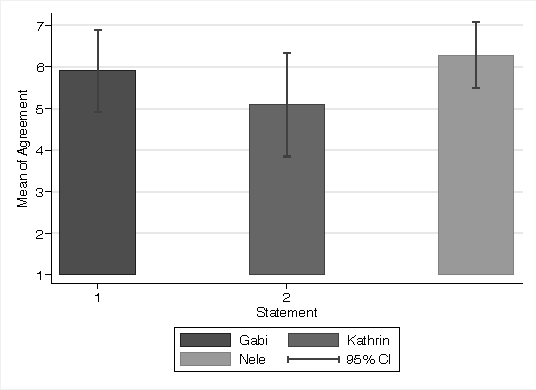
\includegraphics[scale=0.8]{figures/pilot_study_8.pdf}
   \begin{minipage}{0.9\linewidth}
   \footnotesize
   \emph{The figure shows the mean of agreements with the statements ``Kathrin gave Nele juice with a sippy cup that was poisoned because Gabi had poisoned Nele's sippy cup'', ``Nele ingested poison because Kathrin gave Nele juice with a sippy cup that was poisoned'', and ``Nele died because she ingested poison''. $N=21$.}
   \end{minipage}
   \caption{Mean of agreements in Pilot Study 8}
   \label{fig:pilot_study_8}
\end{figure}

\noindent To sum up, the outlook from Studies 1 and 2 served as a first indicator that the results from L\&S (2020) should be replicable with a German sample. Studies 2 and 3 hinted at a possible success of the IOC Exclusion, with Study 3 giving a first indication that omitting the agents' names might have a significant influence. Studies 4 and 5, then, hinted at a possible success of the CRC Exclusion. For the main experiment, we limited ourselves to a single study in which we altered the phrasing to the usual structure used for counterfactual conditionals. Study 6 hinted at a success of the CEQ Exclusion. Lastly, Studies 7 and 8 provided reason to believe that a combination of the aforementioned approaches might be successful. As we did for the CRC Exclusion, we limited ourselves to a single study for the main experiment.

\clearpage
\section{Additional Texts}\label{app:main_instructions}
\subsection{Welcome Message}\label{app:main_welcome}
Welcome to our study!%Herzlich willkommen zu unserer Studie!
	
If you focus on the task, you will probably need no more than five to ten minutes for this study. It is important that you read the instructions carefully. Also, please complete the study without closing your browser in between.%Bei konzentrierter Bearbeitung werden Sie voraussichtlich nicht länger als fünf bis zehn Minuten für diese Studie benötigen. Es ist wichtig, dass Sie die Hinweise und Aufgaben aufmerksam lesen. Bearbeiten Sie die Studie bitte außerdem, ohne den Browser zwischendurch zu schließen.
	
We will evaluate your assessment as well as the assessments of all other participants in this study. All data will be stored in anonymized form so that no information can be assigned to an individual person. The results of the study will be published.%Wir werden Ihre Einschätzungen sowie die Einschätzungen aller anderen Teilnehmerinnen und Teilnehmer dieser Studie auswerten. Alle Daten werden in anonymisierter Form gespeichert, so dass keine Angaben einer einzelnen Person zugeordnet werden können. Die Ergebnisse der Studie werden veröffentlicht.
	
Thank you for your participation!%Vielen Dank für Ihre Teilnahme!

\subsection{Control Questions for Poisoned Cup Vignette}\label{app:main_cup_control}
\noindent\textit{Note: Question 3 was only posed to subjects of studies 4 and 6 on the Poisoned Cup Vignette (Sections \ref{sec:results_cup_crc} and \ref{sec:results_cup_com}).}

\vspace{1ex}
\noindent\textbf{Question 1:} Did Kathrin poison Nele's sippy cup?%Hat Kathrin Neles Trinkbecher vergiftet?

\vspace{1ex}
\noindent\textbf{Question 2:} Did Gabi give Nele the poisoned sippy cup?%Hat Gabi Nele den vergifteten Trinkbecher gegeben?

\vspace{1ex}
\noindent\textbf{Question 3:} There would be no alternation of day and night if the earth did not revolve around itself.%Es gäbe nicht den Wechsel von Tag und Nacht, wenn sich die Erde nicht um sich selbst drehen würde.

\subsection{Control Questions for Revolver Vignette}\label{app:main_revolver_control}
\noindent\textit{Note: Question 3 was only posed to subjects of studies 3 and 5 on the Revolver Vignette (Sections \ref{sec:results_rev_crc} and \ref{sec:results_rev_com}).}

\vspace{1ex}
\noindent\textbf{Question 1:} Did Uwe pull the trigger?%Hat Uwe den Abzug gedrückt?

\vspace{1ex}
\noindent\textbf{Question 2:} Is Leeve Uwe's father?%Ist Leeve Uwes Vater?

\vspace{1ex}
\noindent\textbf{Question 3:} There would be no alternation of day and night if the earth did not revolve around itself.%Es gäbe nicht den Wechsel von Tag und Nacht, wenn sich die Erde nicht um sich selbst drehen würde.

\subsection{Control Questions for GFCI Vignette}\label{app:main_circuit_control}
\noindent\textit{Note: Question 3 was only posed to subjects of studies 3 and 5 on the GFCI Vignette (Sections \ref{sec:results_cir_crc} and \ref{sec:results_cir_com}).}

\vspace{1ex}
\noindent\textbf{Question 1:} Did Mark conduct an experiment with an unusual species of insect?%Hat Mark ein Experiment mit einer ungewöhnlichen Insektenart durchgeführt?

\vspace{1ex}
\noindent\textbf{Question 2:} Has water gotten into the socket?%Ist Wasser in die Steckdose gelangt?

\vspace{1ex}
\noindent\textbf{Question 3:} There would be no alternation of day and night if the earth did not revolve around itself.%Es gäbe nicht den Wechsel von Tag und Nacht, wenn sich die Erde nicht um sich selbst drehen würde.

\clearpage
\section{Additional Figures}\label{app:additional_figures}
\subsection{Poisoned Cup Vignette –- Replication}
\begin{figure}[H]
   \centering
   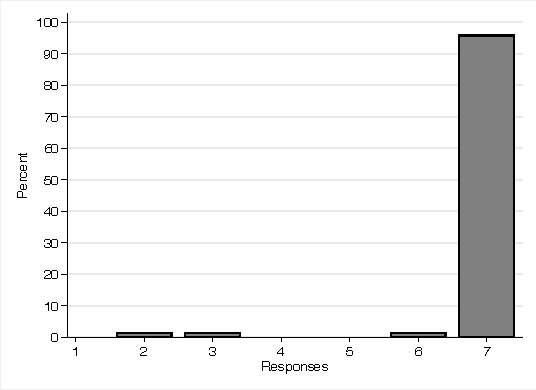
\includegraphics[scale=0.8]{figures/cup_rep_hist_1.pdf}
   \begin{minipage}{0.9\linewidth}
   \footnotesize
   \emph{The figure shows the relative frequencies of answers to the statement ``Gabi caused Nele's death''. $N=71$.}
   \end{minipage}
   \caption{Relative frequencies for statement 1 in the replication with Poisoned Cup Vignette}
   \label{fig:cup_rep_hist_1}
\end{figure}

\begin{figure}[H]
   \centering
   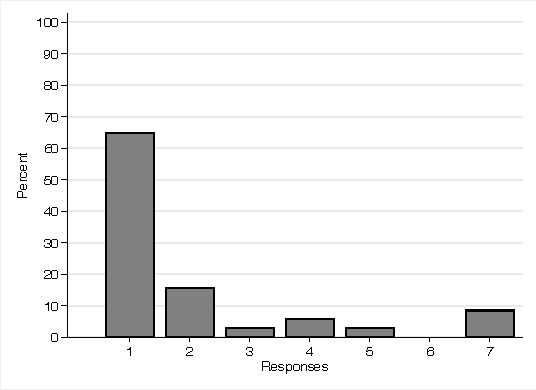
\includegraphics[scale=0.8]{figures/cup_rep_hist_2.pdf}
   \begin{minipage}{0.9\linewidth}
   \footnotesize
   \emph{The figure shows the relative frequencies of answers to the statement ``Kathrin caused Nele's death''. $N=71$.}
   \end{minipage}
   \caption{Relative frequencies for statement 2 in the replication with Poisoned Cup Vignette}
   \label{fig:cup_rep_hist_2}
\end{figure}

\subsection{Poisoned Cup Vignette –- IOC Exclusion (1)}
\begin{figure}[H]
   \centering
   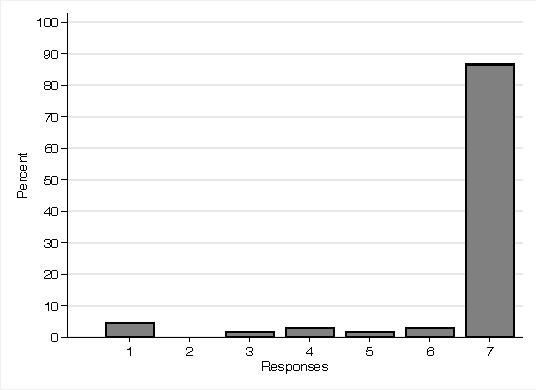
\includegraphics[scale=0.8]{figures/cup_ioc_1_hist_1.pdf}
   \begin{minipage}{0.9\linewidth}
   \footnotesize
   \emph{The figure shows the relative frequencies of answers to the statement ``Gabis's action of poisoning the sippy cup caused Nele's death''. $N=67$.}
   \end{minipage}
   \caption{Relative frequencies for statement 1 in IOC Exclusion (1) with Poisoned Cup Vignette}
   \label{fig:cup_ioc_1_hist_1}
\end{figure}

\begin{figure}[H]
   \centering
   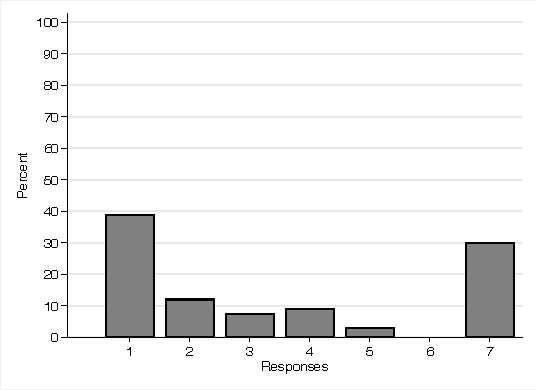
\includegraphics[scale=0.8]{figures/cup_ioc_1_hist_2.pdf}
   \begin{minipage}{0.9\linewidth}
   \footnotesize
   \emph{The figure shows the relative frequencies of answers to the statement ``Kathrin's action of giving Nele a poisoned sippy cup caused Nele's death''. $N=67$.}
   \end{minipage}
   \caption{Relative frequencies for statement 2 in IOC Exclusion (1) with Poisoned Cup Vignette}
   \label{fig:cup_ioc_1_hist_2}
\end{figure}

\subsection{Poisoned Cup Vignette –- IOC Exclusion (2)}
\begin{figure}[H]
   \centering
   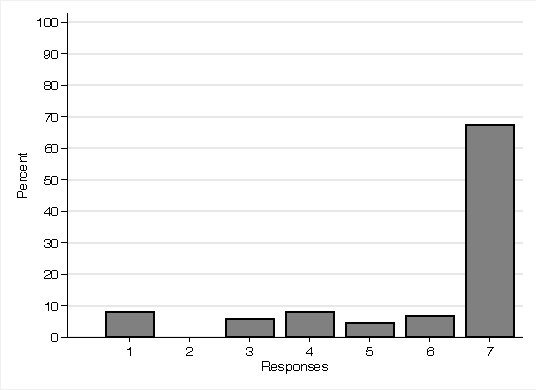
\includegraphics[scale=0.8]{figures/cup_ioc_2_hist_1.pdf}
   \begin{minipage}{0.9\linewidth}
   \footnotesize
   \emph{The figure shows the relative frequencies of answers to the statement ``The action of poisoning the sippy cup caused Nele's death''. $N=81$.}
   \end{minipage}
   \caption{Relative frequencies for statement 1 in IOC Exclusion (2) with Poisoned Cup Vignette}
   \label{fig:cup_ioc_2_hist_1}
\end{figure}

\begin{figure}[H]
   \centering
   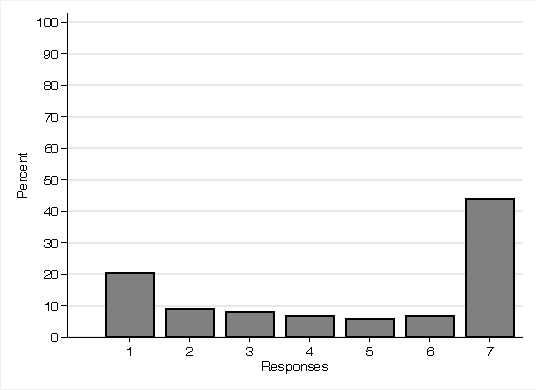
\includegraphics[scale=0.8]{figures/cup_ioc_2_hist_2.pdf}
   \begin{minipage}{0.9\linewidth}
   \footnotesize
   \emph{The figure shows the relative frequencies of answers to the statement ``The action of giving Nele juice with a poisoned sippy cup caused Nele's death''. $N=81$.}
   \end{minipage}
   \caption{Relative frequencies for statement 2 in IOC Exclusion (2) with Poisoned Cup Vignette}
   \label{fig:cup_ioc_2_hist_2}
\end{figure}

\subsection{Poisoned Cup Vignette –- CRC Exclusion}
\begin{figure}[H]
   \centering
   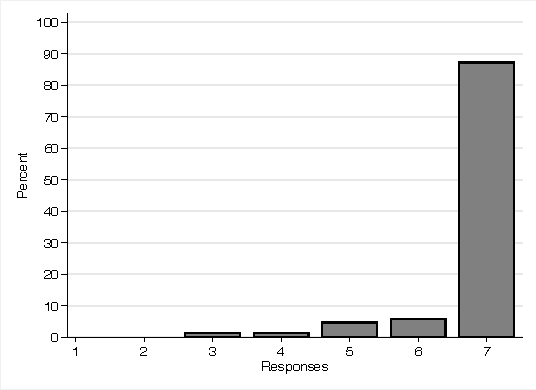
\includegraphics[scale=0.8]{figures/cup_crc_hist_1.pdf}
   \begin{minipage}{0.9\linewidth}
   \footnotesize
   \emph{The figure shows the relative frequencies of answers to the statement ``Nele would not have died that evening if Gabi had not poisoned her sippy cup''. $N=86$.}
   \end{minipage}
   \caption{Relative frequencies for statement 1 in CRC Exclusion with Poisoned Cup Vignette}
   \label{fig:cup_crc_hist_1}
\end{figure}

\begin{figure}[H]
   \centering
   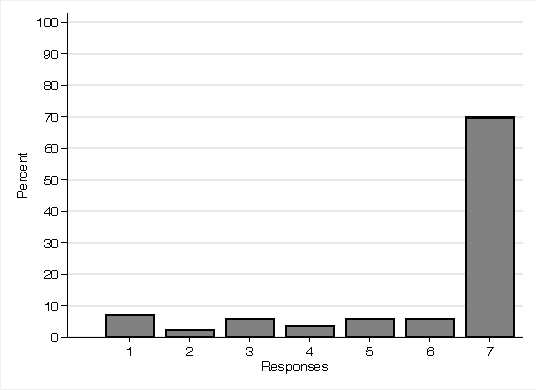
\includegraphics[scale=0.8]{figures/cup_crc_hist_2.pdf}
   \begin{minipage}{0.9\linewidth}
   \footnotesize
   \emph{The figure shows the relative frequencies of answers to the statement ``Nele would not have died that evening if Kathrin had not given her juice in a poisoned sippy cup''. $N=86$.}
   \end{minipage}
   \caption{Relative frequencies for statement 2 in CRC Exclusion with Poisoned Cup Vignette}
   \label{fig:cup_crc_hist_2}
\end{figure}

\subsection{Poisoned Cup Vignette –- CEQ Exclusion}
\begin{figure}[H]
   \centering
   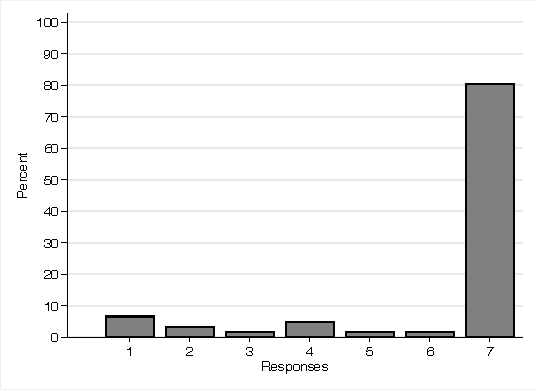
\includegraphics[scale=0.8]{figures/cup_ceq_hist_1.pdf}
   \begin{minipage}{0.9\linewidth}
   \footnotesize
   \emph{The figure shows the relative frequencies of answers to the statement ``Gabi's action of poisoning Nele's sippy cup caused Kathrin to give Nele juice in a poisoned sippy cup''. $N=61$.}
   \end{minipage}
   \caption{Relative frequencies for statement 1 in CEQ Exclusion with Poisoned Cup Vignette}
   \label{fig:cup_ceq_hist_1}
\end{figure}

\begin{figure}[H]
   \centering
   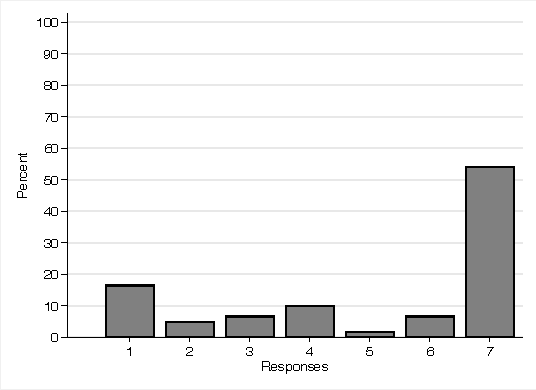
\includegraphics[scale=0.8]{figures/cup_ceq_hist_2.pdf}
   \begin{minipage}{0.9\linewidth}
   \footnotesize
   \emph{The figure shows the relative frequencies of answers to the statement ``Kathrin's action of giving Nele juice in a poisoned sippy cup caused Nele to ingest poison''. $N=61$.}
   \end{minipage}
   \caption{Relative frequencies for statement 2 in CEQ Exclusion with Poisoned Cup Vignette}
   \label{fig:cup_ceq_hist_2}
\end{figure}

\begin{figure}[H]
   \centering
   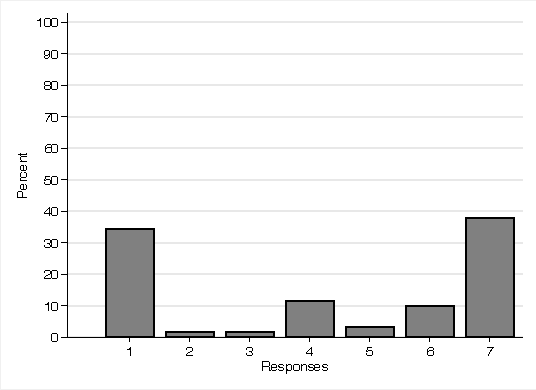
\includegraphics[scale=0.8]{figures/cup_ceq_hist_3.pdf}
   \begin{minipage}{0.9\linewidth}
   \footnotesize
   \emph{The figure shows the relative frequencies of answers to the statement ``Nele's action of ingesting poison caused her death''. $N=61$.}
   \end{minipage}
   \caption{Relative frequencies for statement 3 in CEQ Exclusion with Poisoned Cup Vignette}
   \label{fig:cup_ceq_hist_3}
\end{figure}

\subsection{Poisoned Cup Vignette -- Simultaneous Exclusion}
\begin{figure}[H]
   \centering
   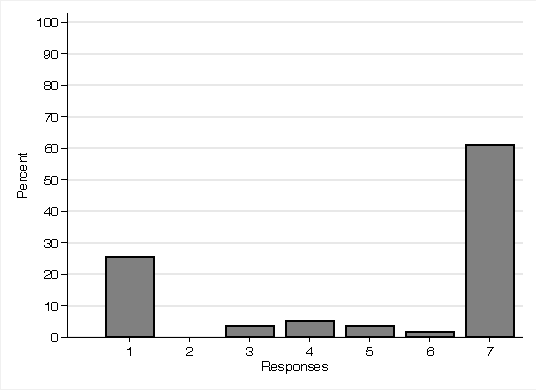
\includegraphics[scale=0.8]{figures/cup_com_hist_1.pdf}
   \begin{minipage}{0.9\linewidth}
   \footnotesize
   \emph{The figure shows the relative frequencies of answers to the statement ``Kathrin would not have given Nele juice in a poisoned sippy cup if Gabi had not poisoned Nele's sippy cup''. $N=59$.}
   \end{minipage}
   \caption{Relative frequencies for statement 1 in simultaneous IOC, CRC, and CEQ Exclusion with Poisoned Cup Vignette}
   \label{fig:cup_com_hist_1}
\end{figure}

\begin{figure}[H]
   \centering
   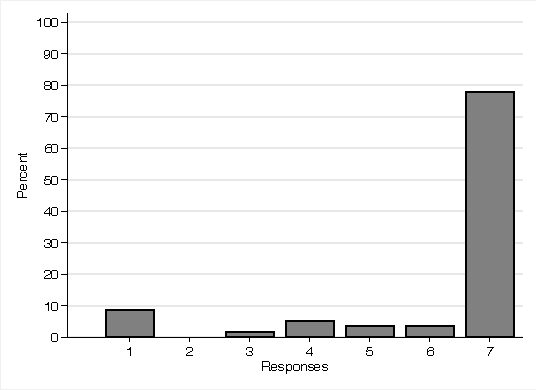
\includegraphics[scale=0.8]{figures/cup_com_hist_2.pdf}
   \begin{minipage}{0.9\linewidth}
   \footnotesize
   \emph{The figure shows the relative frequencies of answers to the statement ``Nele would not have ingested poison if Kathrin had not given her juice in a poisoned sippy cup''. $N=59$.}
   \end{minipage}
   \caption{Relative frequencies for statement 2 in simultaneous IOC, CRC, and CEQ Exclusion with Poisoned Cup Vignette}
   \label{fig:cup_com_hist_2}
\end{figure}

\begin{figure}[H]
   \centering
   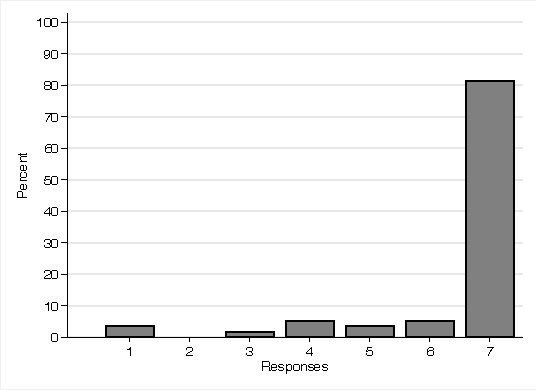
\includegraphics[scale=0.8]{figures/cup_com_hist_3.pdf}
   \begin{minipage}{0.9\linewidth}
   \footnotesize
   \emph{The figure shows the relative frequencies of answers to the statement ``Nele would not have died that evening if she had not ingested the poison''. $N=59$.}
   \end{minipage}
   \caption{Relative frequencies for statement 3 in simultaneous IOC, CRC, and CEQ Exclusion with Poisoned Cup Vignette}
   \label{fig:cup_com_hist_3}
\end{figure}

\subsection{Revolver Vignette -- Replication}
\begin{figure}[H]
   \centering
   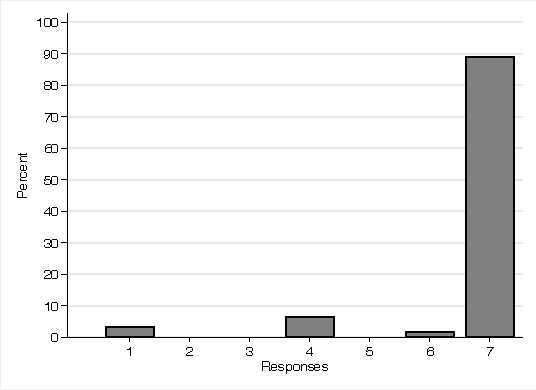
\includegraphics[scale=0.8]{figures/rev_rep_hist_1.pdf}
   \begin{minipage}{0.9\linewidth}
   \footnotesize
   \emph{The figure shows the relative frequencies of answers to the statement ``Leeve caused Uwe's death''. $N=63$.}
   \end{minipage}
   \caption{Relative frequencies for statement 1 in replication with Revolver Vignette}
   \label{fig:rev_rep_hist_1}
\end{figure}

\begin{figure}[H]
   \centering
   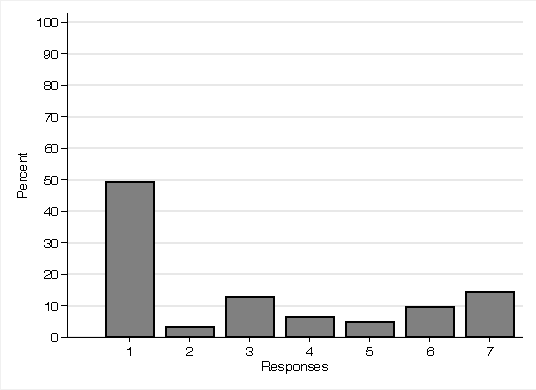
\includegraphics[scale=0.8]{figures/rev_rep_hist_2.pdf}
   \begin{minipage}{0.9\linewidth}
   \footnotesize
   \emph{The figure shows the relative frequencies of answers to the statement ``The hammer caused Uwe's death''. $N=63$.}
   \end{minipage}
   \caption{Relative frequencies for statement 2 in replication with Revolver Vignette}
   \label{fig:rev_rep_hist_2}
\end{figure}

\begin{figure}[H]
   \centering
   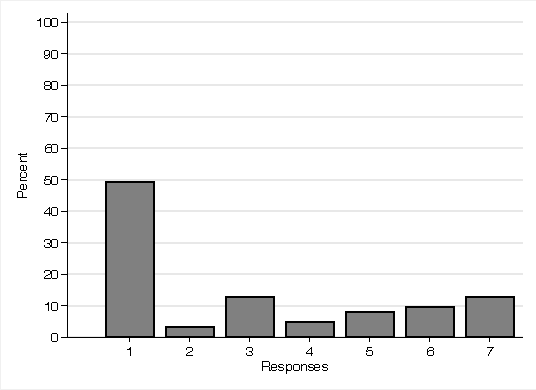
\includegraphics[scale=0.8]{figures/rev_rep_hist_3.pdf}
   \begin{minipage}{0.9\linewidth}
   \footnotesize
   \emph{The figure shows the relative frequencies of answers to the statement ``The gun powder caused Uwe's death''. $N=63$.}
   \end{minipage}
   \caption{Relative frequencies for statement 3 in replication with Revolver Vignette}
   \label{fig:rev_rep_hist_3}
\end{figure}

\begin{figure}[H]
   \centering
   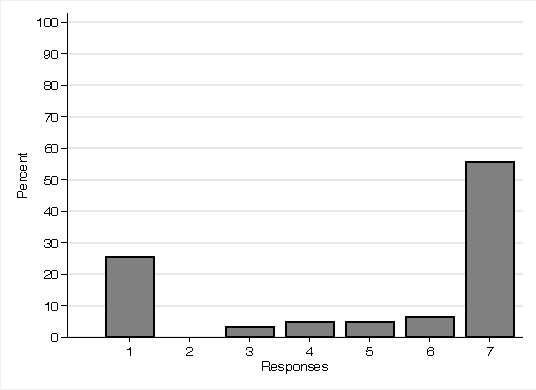
\includegraphics[scale=0.8]{figures/rev_rep_hist_4.pdf}
   \begin{minipage}{0.9\linewidth}
   \footnotesize
   \emph{The figure shows the relative frequencies of answers to the statement ``The bullet caused Uwe's death''. $N=63$.}
   \end{minipage}
   \caption{Relative frequencies for statement 4 in replication with Revolver Vignette}
   \label{fig:rev_rep_hist_4}
\end{figure}

\subsection{Revolver Vignette -- IOC Exclusion}
\begin{figure}[H]
   \centering
   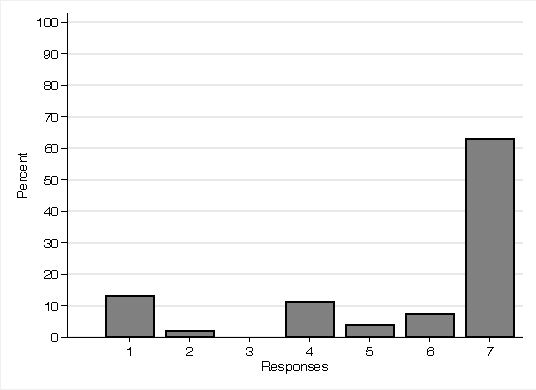
\includegraphics[scale=0.8]{figures/rev_ioc_hist_1.pdf}
   \begin{minipage}{0.9\linewidth}
   \footnotesize
   \emph{The figure shows the relative frequencies of answers to the statement ``Leeve's action of shooting at Uwe caused Uwe's death''. $N=54$.}
   \end{minipage}
   \caption{Relative frequencies for statement 1 in IOC Exclusion with Revolver Vignette}
   \label{fig:rev_ioc_hist_1}
\end{figure}

\begin{figure}[H]
   \centering
   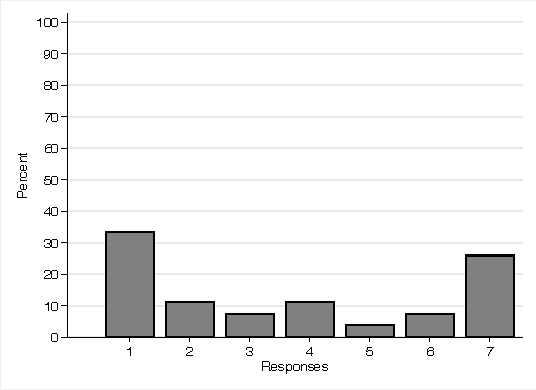
\includegraphics[scale=0.8]{figures/rev_ioc_hist_2.pdf}
   \begin{minipage}{0.9\linewidth}
   \footnotesize
   \emph{The figure shows the relative frequencies of answers to the statement ``The release of the hammer caused Uwe's death''. $N=54$.}
   \end{minipage}
   \caption{Relative frequencies for statement 2 in IOC Exclusion with Revolver Vignette}
   \label{fig:rev_ioc_hist_2}
\end{figure}

\begin{figure}[H]
   \centering
   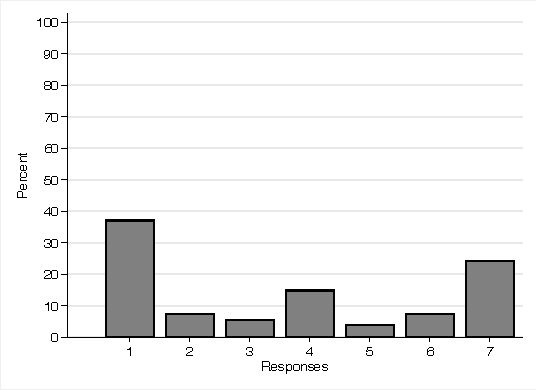
\includegraphics[scale=0.8]{figures/rev_ioc_hist_3.pdf}
   \begin{minipage}{0.9\linewidth}
   \footnotesize
   \emph{The figure shows the relative frequencies of answers to the statement ``The explosion of the gun powder caused Uwe's death''. $N=54$.}
   \end{minipage}
   \caption{Relative frequencies for statement 3 in IOC Exclusion with Revolver Vignette}
   \label{fig:rev_ioc_hist_3}
\end{figure}

\begin{figure}[H]
   \centering
   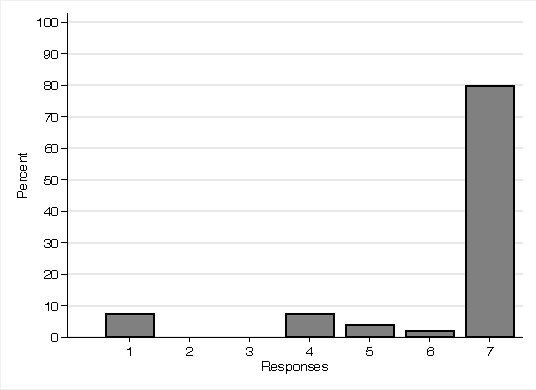
\includegraphics[scale=0.8]{figures/rev_ioc_hist_4.pdf}
   \begin{minipage}{0.9\linewidth}
   \footnotesize
   \emph{The figure shows the relative frequencies of answers to the statement ``The bullet hitting Uwe caused Uwe's death''. $N=54$.}
   \end{minipage}
   \caption{Relative frequencies for statement 4 in IOC Exclusion with Revolver Vignette}
   \label{fig:rev_ioc_hist_4}
\end{figure}

\subsection{Revolver Vignette -- CRC Exclusion}
\begin{figure}[H]
   \centering
   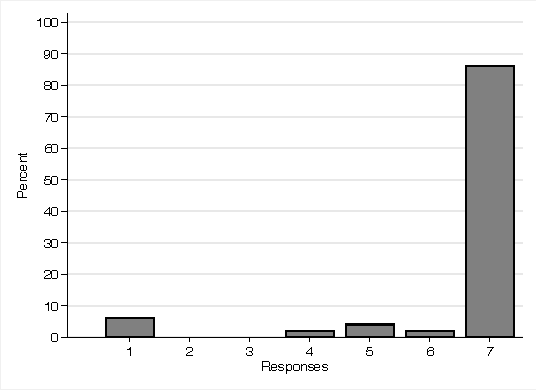
\includegraphics[scale=0.8]{figures/rev_crc_hist_1.pdf}
   \begin{minipage}{0.9\linewidth}
   \footnotesize
   \emph{The figure shows the relative frequencies of answers to the statement ``Uwe would not have died if Leeve had not shot at him''. $N=54$.}
   \end{minipage}
   \caption{Relative frequencies for statement 1 in CRC Exclusion with Revolver Vignette}
   \label{fig:rev_crc_hist_1}
\end{figure}

\begin{figure}[H]
   \centering
   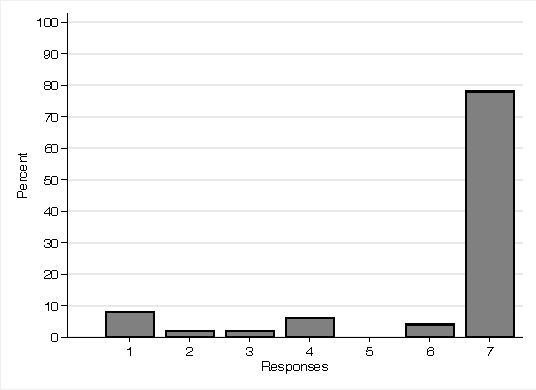
\includegraphics[scale=0.8]{figures/rev_crc_hist_2.pdf}
   \begin{minipage}{0.9\linewidth}
   \footnotesize
   \emph{The figure shows the relative frequencies of answers to the statement ``Uwe would not have died if the hammer had not been released''. $N=54$.}
   \end{minipage}
   \caption{Relative frequencies for statement 2 in CRC Exclusion with Revolver Vignette}
   \label{fig:rev_crc_hist_2}
\end{figure}

\begin{figure}[H]
   \centering
   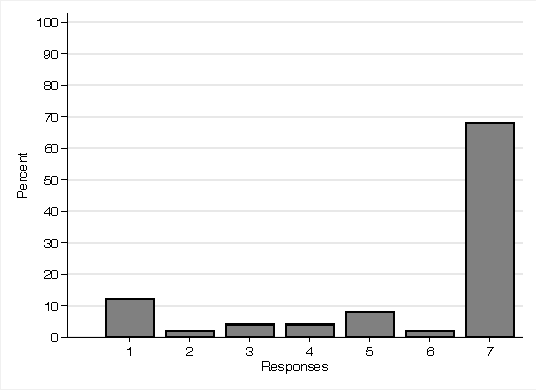
\includegraphics[scale=0.8]{figures/rev_crc_hist_3.pdf}
   \begin{minipage}{0.9\linewidth}
   \footnotesize
   \emph{The figure shows the relative frequencies of answers to the statement ``Uwe would not have died if the gun powder had not exploded''. $N=54$.}
   \end{minipage}
   \caption{Relative frequencies for statement 3 in CRC Exclusion with Revolver Vignette}
   \label{fig:rev_crc_hist_3}
\end{figure}

\begin{figure}[H]
   \centering
   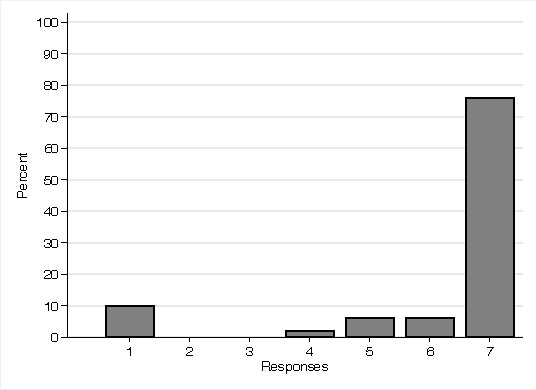
\includegraphics[scale=0.8]{figures/rev_crc_hist_4.pdf}
   \begin{minipage}{0.9\linewidth}
   \footnotesize
   \emph{The figure shows the relative frequencies of answers to the statement ``Uwe would not have died if the bullet had not hit Uwe''. $N=54$.}
   \end{minipage}
   \caption{Relative frequencies for statement 4 in CRC Exclusion with Revolver Vignette}
   \label{fig:rev_crc_hist_4}
\end{figure}

\subsection{Revolver Vignette -- CEQ Exclusion}
\begin{figure}[H]
   \centering
   \includegraphics[scale=0.8]{figures/rev_ceq_hist_1.pdf}
   \begin{minipage}{0.9\linewidth}
   \footnotesize
   \emph{The figure shows the relative frequencies of answers to the statement ``Leeve's action of shooting at Uwe caused the release of the hammer''. $N=53$.}
   \end{minipage}
   \caption{Relative frequencies for statement 1 in CEQ Exclusion with Revolver Vignette}
   \label{fig:rev_ceq_hist_1}
\end{figure}

\begin{figure}[H]
   \centering
   \includegraphics[scale=0.8]{figures/rev_ceq_hist_2.pdf}
   \begin{minipage}{0.9\linewidth}
   \footnotesize
   \emph{The figure shows the relative frequencies of answers to the statement ``The release of the hammer caused the explosion of the gun powder''. $N=53$.}
   \end{minipage}
   \caption{Relative frequencies for statement 2 in CEQ Exclusion with Revolver Vignette}
   \label{fig:rev_ceq_hist_2}
\end{figure}

\begin{figure}[H]
   \centering
   \includegraphics[scale=0.8]{figures/rev_ceq_hist_3.pdf}
   \begin{minipage}{0.9\linewidth}
   \footnotesize
   \emph{The figure shows the relative frequencies of answers to the statement ``The explosion of the gun powder caused the bullet to hit Uwe''. $N=53$.}
   \end{minipage}
   \caption{Relative frequencies for statement 3 in CEQ Exclusion with Revolver Vignette}
   \label{fig:rev_ceq_hist_3}
\end{figure}

\begin{figure}[H]
   \centering
   \includegraphics[scale=0.8]{figures/rev_ceq_hist_4.pdf}
   \begin{minipage}{0.9\linewidth}
   \footnotesize
   \emph{The figure shows the relative frequencies of answers to the statement ``The bullet hitting Uwe caused Uwe's death''. $N=53$.}
   \end{minipage}
   \caption{Relative frequencies for statement 4 in CEQ Exclusion with Revolver Vignette}
   \label{fig:rev_ceq_hist_4}
\end{figure}

\subsection{Revolver Vignette -- Simulatneous Exclusion}
\begin{figure}[H]
   \centering
   \includegraphics[scale=0.8]{figures/rev_com_hist_1.pdf}
   \begin{minipage}{0.9\linewidth}
   \footnotesize
   \emph{The figure shows the relative frequencies of answers to the statement ``The hammer would not have released if Leeve had not shot at Uwe''. $N=50$.}
   \end{minipage}
   \caption{Relative frequencies for statement 1 in Simultaneous IOC, CRC, and CEQ Exclusion with Revolver Vignette}
   \label{fig:rev_com_hist_1}
\end{figure}

\begin{figure}[H]
   \centering
   \includegraphics[scale=0.8]{figures/rev_com_hist_2.pdf}
   \begin{minipage}{0.9\linewidth}
   \footnotesize
   \emph{The figure shows the relative frequencies of answers to the statement ``The gun powder would not have exploded if the hammer had not released''. $N=50$.}
   \end{minipage}
   \caption{Relative frequencies for statement 2 in Simultaneous IOC, CRC, and CEQ Exclusion with Revolver Vignette}
   \label{fig:rev_com_hist_2}
\end{figure}

\begin{figure}[H]
   \centering
   \includegraphics[scale=0.8]{figures/rev_com_hist_3.pdf}
   \begin{minipage}{0.9\linewidth}
   \footnotesize
   \emph{The figure shows the relative frequencies of answers to the statement ``The bullet would not have hit Uwe if the gun powder had not exploded''. $N=50$.}
   \end{minipage}
   \caption{Relative frequencies for statement 3 in Simultaneous IOC, CRC, and CEQ Exclusion with Revolver Vignette}
   \label{fig:rev_com_hist_3}
\end{figure}

\begin{figure}[H]
   \centering
   \includegraphics[scale=0.8]{figures/rev_com_hist_4.pdf}
   \begin{minipage}{0.9\linewidth}
   \footnotesize
   \emph{The figure shows the relative frequencies of answers to the statement ``Uwe would not have died if the bullet had not hit Uwe''. $N=50$.}
   \end{minipage}
   \caption{Relative frequencies for statement 4 in Simultaneous IOC, CRC, and CEQ Exclusion with Revolver Vignette}
   \label{fig:rev_com_hist_4}
\end{figure}

\subsection{GFCI Vignette -- Replication}
\begin{figure}[H]
   \centering
   \includegraphics[scale=0.8]{figures/cir_rep_hist_1.pdf}
   \begin{minipage}{0.9\linewidth}
   \footnotesize
   \emph{The figure shows the relative frequencies of answers to the statement ``The pipe bursting caused the experiment to be ruined''. $N=60$.}
   \end{minipage}
   \caption{Relative frequencies for statement 1 in replication with GFCI Vignette}
   \label{fig:cir_rep_hist_1}
\end{figure}

\begin{figure}[H]
   \centering
   \includegraphics[scale=0.8]{figures/cir_rep_hist_2.pdf}
   \begin{minipage}{0.9\linewidth}
   \footnotesize
   \emph{The figure shows the relative frequencies of answers to the statement ``The GFCI breaking the circuit caused the experiment to be ruined''. $N=60$.}
   \end{minipage}
   \caption{Relative frequencies for statement 2 in replication with GFCI Vignette}
   \label{fig:cir_rep_hist_2}
\end{figure}

\subsection{GFCI Vignette -- IOC Exclusion}
\begin{figure}[H]
   \centering
   \includegraphics[scale=0.8]{figures/cir_ioc_hist_1.pdf}
   \begin{minipage}{0.9\linewidth}
   \footnotesize
   \emph{The figure shows the relative frequencies of answers to the statement ``The pipe bursting caused the experiment to be ruined''. $N=64$.}
   \end{minipage}
   \caption{Relative frequencies for statement 1 in IOC Exclusion with GFCI Vignette}
   \label{fig:cir_ioc_hist_1}
\end{figure}

\begin{figure}[H]
   \centering
   \includegraphics[scale=0.8]{figures/cir_ioc_hist_2.pdf}
   \begin{minipage}{0.9\linewidth}
   \footnotesize
   \emph{The figure shows the relative frequencies of answers to the statement ``The breaking of the circuit by the GFCI caused the experiment to be ruined''. $N=64$.}
   \end{minipage}
   \caption{Relative frequencies for statement 2 in IOC Exclusion with GFCI Vignette}
   \label{fig:cir_ioc_hist_2}
\end{figure}

\subsection{GFCI Vignette -- CRC Exclusion}
\begin{figure}[H]
   \centering
   \includegraphics[scale=0.8]{figures/cir_crc_hist_1.pdf}
   \begin{minipage}{0.9\linewidth}
   \footnotesize
   \emph{The figure shows the relative frequencies of answers to the statement ``The experiment would not have been ruined if the pipe had not burst''. $N=67$.}
   \end{minipage}
   \caption{Relative frequencies for statement 1 in CRC Exclusion with GFCI Vignette}
   \label{fig:cir_crc_hist_1}
\end{figure}

\begin{figure}[H]
   \centering
   \includegraphics[scale=0.8]{figures/cir_crc_hist_2.pdf}
   \begin{minipage}{0.9\linewidth}
   \footnotesize
   \emph{The figure shows the relative frequencies of answers to the statement ``The experiment would not have been ruined if the GFCI had not broken the circuit''. $N=67$.}
   \end{minipage}
   \caption{Relative frequencies for statement 2 in CRC Exclusion with GFCI Vignette}
   \label{fig:cir_crc_hist_2}
\end{figure}

\subsection{GFCI Vignette -- CEQ Exclusion}
\begin{figure}[H]
   \centering
   \includegraphics[scale=0.8]{figures/cir_ceq_hist_1.pdf}
   \begin{minipage}{0.9\linewidth}
   \footnotesize
   \emph{The figure shows the relative frequencies of answers to the statement ``The bursting of the pipe caused the GFCI to break to circuit''. $N=64$.}
   \end{minipage}
   \caption{Relative frequencies for statement 1 in CEQ Exclusion with GFCI Vignette}
   \label{fig:cir_ceq_hist_1}
\end{figure}

\begin{figure}[H]
   \centering
   \includegraphics[scale=0.8]{figures/cir_ceq_hist_2.pdf}
   \begin{minipage}{0.9\linewidth}
   \footnotesize
   \emph{The figure shows the relative frequencies of answers to the statement ``The breaking of the circuit by the GFCI caused the special light to turn off''. $N=64$.}
   \end{minipage}
   \caption{Relative frequencies for statement 2 in CEQ Exclusion with GFCI Vignette}
   \label{fig:cir_ceq_hist_2}
\end{figure}

\begin{figure}[H]
   \centering
   \includegraphics[scale=0.8]{figures/cir_ceq_hist_3.pdf}
   \begin{minipage}{0.9\linewidth}
   \footnotesize
   \emph{The figure shows the relative frequencies of answers to the statement ``The special light turning off caused the experiment to be ruined''. $N=64$.}
   \end{minipage}
   \caption{Relative frequencies for statement 3 in CEQ Exclusion with GFCI Vignette}
   \label{fig:cir_ceq_hist_3}
\end{figure}

\subsection{GFCI Vignette -- Simultaneous Exclusion}
\begin{figure}[H]
   \centering
   \includegraphics[scale=0.8]{figures/cir_com_hist_1.pdf}
   \begin{minipage}{0.9\linewidth}
   \footnotesize
   \emph{The figure shows the relative frequencies of answers to the statement ``The GFCI would not have broken the circuit if the pipe had not burst''. $N=59$.}
   \end{minipage}
   \caption{Relative frequencies for statement 1 in simultaneous IOC, CRC, and CEQ Exclusion with GFCI Vignette}
   \label{fig:cir_com_hist_1}
\end{figure}

\begin{figure}[H]
   \centering
   \includegraphics[scale=0.8]{figures/cir_com_hist_2.pdf}
   \begin{minipage}{0.9\linewidth}
   \footnotesize
   \emph{The figure shows the relative frequencies of answers to the statement ``The special light would not have turned off if the GFCI had not broken the circuit''. $N=59$.}
   \end{minipage}
   \caption{Relative frequencies for statement 2 in simultaneous IOC, CRC, and CEQ Exclusion with GFCI Vignette}
   \label{fig:cir_com_hist_2}
\end{figure}

\begin{figure}[H]
   \centering
   \includegraphics[scale=0.8]{figures/cir_com_hist_3.pdf}
   \begin{minipage}{0.9\linewidth}
   \footnotesize
   \emph{The figure shows the relative frequencies of answers to the statement ``The experiment would not have been ruined if the special light had not turned off''. $N=59$.}
   \end{minipage}
   \caption{Relative frequencies for statement 3 in simultaneous IOC, CRC, and CEQ Exclusion with GFCI Vignette}
   \label{fig:cir_com_hist_3}
\end{figure}

\end{document}
